% !TeX program = pdflatex
% !TeX encoding = UTF-8
\documentclass[11pt,aspectratio=169,t]{beamer}
% Все презентации курса компилируются только pdflatex.
\usepackage{iftex}
\RequirePDFTeX
\usepackage{cmap}
\usepackage[T2A]{fontenc}
\usepackage[utf8]{inputenc}
\usepackage[english,russian]{babel}
\usepackage{PTSerif}
\usepackage{amsmath,amsfonts,amssymb}
\usepackage{graphicx,microtype,anyfontsize,tikz}
\usepackage{ragged2e}
\usetikzlibrary{arrows.meta,calc}

\usetheme{default}
\usefonttheme{serif}
\DeclareMathOperator{\sen}{sen}
\bibliographystyle{apalike}

% Общие сведения; номер лекции, её название и дата задаются в N.tex.
\newcommand{\coursename}{Введение в маневрирование КА}
\author{Чиняев Владимир Николаевич}
\institute{Московский физико-технический институт}

% Книжное оформление с голубым акцентом.
\definecolor{coursepaper}{HTML}{FBF9F3}
\definecolor{courseink}{HTML}{302B28}
\definecolor{courseaccent}{HTML}{187AA5}
\definecolor{coursemuted}{HTML}{6D6560}
\definecolor{courserule}{HTML}{A9CADA}
\definecolor{coursetint}{HTML}{EDF4F6}
\tikzset{
  course diagram/.style={font=\fontsize{9.5}{11.5}\selectfont,
    line cap=round,line join=round,>=Latex},
  orbit line/.style={draw=courseaccent,line width=1pt},
  aux line/.style={draw=courserule,line width=.5pt},
  vector line/.style={draw=courseink,line width=.65pt,->},
  angle line/.style={draw=courseaccent,line width=.8pt,->},
  orbit point/.style={circle,fill=courseaccent,inner sep=1.7pt}
}
\setbeamercolor{normal text}{fg=courseink,bg=coursepaper}
\setbeamercolor{background canvas}{bg=coursepaper}
\setbeamercolor{structure}{fg=courseaccent}
\setbeamercolor{alerted text}{fg=courseaccent}
\setbeamercolor{frametitle}{fg=courseink,bg=coursepaper}
\setbeamercolor{footline}{fg=coursemuted,bg=coursepaper}
\setbeamercolor{caption name}{fg=courseaccent}

% Основной текст — 11/14 pt; подписи к рисункам — 9.5/11.5 pt.
\let\coursenormalsize\normalsize
\renewcommand{\normalsize}{\coursenormalsize\fontsize{11}{14}\selectfont}
\setbeamerfont{normal text}{size*={11pt}{14pt}}
\setbeamerfont{frametitle}{size*={20pt}{23pt},series=\mdseries}
\setbeamerfont{title}{size*={27pt}{31pt},series=\mdseries}
\setbeamerfont{subtitle}{size*={12.8pt}{15pt},series=\mdseries}
\setbeamerfont{author}{size*={10.8pt}{13pt}}
\setbeamerfont{institute}{size*={9.2pt}{11pt}}
\setbeamerfont{date}{size*={9pt}{11pt}}
\setbeamerfont{footline}{size*={6.8pt}{8pt}}
\setbeamerfont{caption}{size*={9.5pt}{11.5pt}}
\setbeamerfont{itemize/enumerate body}{size*={11pt}{14pt}}
\setbeamerfont{itemize/enumerate subbody}{size*={11pt}{14pt}}
\setbeamerfont{itemize/enumerate subsubbody}{size*={11pt}{14pt}}
\AtBeginDocument{\normalsize}

\setbeamersize{text margin left=6mm,text margin right=6mm}
\setbeamertemplate{navigation symbols}{}
\setbeamertemplate{headline}{}
\setbeamertemplate{caption}[numbered]
\setbeamertemplate{itemize items}[circle]

% Стандартные блоки Beamer позволяют группировать текст и формулы.
\setbeamertemplate{blocks}[default]
\setbeamerfont{block title}{size*={11pt}{14pt},series=\bfseries}
\setbeamerfont{block body}{size*={11pt}{14pt}}
\setbeamercolor{block title}{fg=courseaccent,bg=coursepaper}
\setbeamercolor{block body}{fg=courseink,bg=coursetint}
\setbeamercolor{block title alerted}{parent=block title}
\setbeamercolor{block body alerted}{parent=block body}
\setbeamercolor{block title example}{parent=block title}
\setbeamercolor{block body example}{parent=block body}

% Компактный заголовок; его высота учитывается при размещении содержания.
\setbeamertemplate{frametitle}{%
  \vskip4.5mm%
  \begin{beamercolorbox}[wd=\textwidth,sep=0pt]{frametitle}
    \usebeamerfont{frametitle}\strut\insertframetitle\strut\par
    \vskip2mm%
    {\color{courseaccent}\hrule height .55pt}
  \end{beamercolorbox}%
}

% Нижний колонтитул: курс слева, лекция и номер слайда справа.
\setbeamertemplate{footline}{%
  \begin{beamercolorbox}[wd=\paperwidth,ht=5.5mm,dp=0pt]{footline}
    \begin{tikzpicture}[remember picture,overlay,x=1mm,y=1mm]
      \begin{scope}[shift={(current page.south west)}]
        \draw[courserule,line width=.3pt] (6,5.5)--(154,5.5);
        \node[text=coursemuted,anchor=west,inner sep=0pt,
          font=\usebeamerfont{footline}] at (6,2.8) {\coursename};
        \node[text=coursemuted,anchor=east,inner sep=0pt,
          font=\usebeamerfont{footline}] at (154,2.8)
          {Лекция \arabic{lecture}\quad\textbullet\quad\insertframenumber};
      \end{scope}
    \end{tikzpicture}%
  \end{beamercolorbox}%
}

% Титульник рассчитан на 16:9 (160 × 90 мм), без нижнего колонтитула.
\setbeamertemplate{title page}{%
  \begin{tikzpicture}[remember picture,overlay,x=1mm,y=1mm]
    \begin{scope}[shift={(current page.south west)}]
      \node[text=coursemuted,anchor=north,font=\usebeamerfont{institute}]
        at (80,82) {\insertinstitute};
      \draw[courseaccent,line width=.55pt] (71,71)--(89,71);
      \node[text=courseink,align=center,text width=125mm,
        font=\usebeamerfont{title}] at (80,53)
        {\hyphenpenalty=10000\coursename\par};
      \node[text=courseaccent,align=center,text width=145mm,font=\usebeamerfont{subtitle}]
        at (80,32) {Лекция \arabic{lecture}. \inserttitle};
      \node[text=courseink,font=\usebeamerfont{author}]
        at (80,19) {\insertauthor};
      \node[text=coursemuted,font=\usebeamerfont{date}]
        at (80,9) {\insertdate};
    \end{scope}
  \end{tikzpicture}%
}

\usepackage{booktabs,array}
\setlength{\abovedisplayskip}{5pt}
\setlength{\belowdisplayskip}{5pt}
\setlength{\abovedisplayshortskip}{3pt}
\setlength{\belowdisplayshortskip}{4pt}
\newcommand{\eqcompact}{\fontsize{10}{12}\selectfont}
\newcommand{\figcaption}[1]{{\usebeamerfont{caption}\color{coursemuted}#1\par}}
\newcommand{\derivationmathspacing}{%
  \setlength{\abovedisplayskip}{2pt}%
  \setlength{\belowdisplayskip}{3pt}%
  \setlength{\abovedisplayshortskip}{2pt}%
  \setlength{\belowdisplayshortskip}{2pt}%
  \setlength{\jot}{2pt}}
\newcommand{\vect}[1]{\boldsymbol{#1}}
\setcounter{lecture}{7}
\title{Задача встречи.\\Задача Ламберта. Относительное движение}
\date{3 ноября 2026 г.}
% Generated by numerics.py. Values use km, s and classical elements.
\newcommand{\ExampleDuration}{1200\,\text{с}}
\newcommand{\ExampleInitialDistance}{2.859\,\text{км}}
\newcommand{\ExampleLinearCost}{4.4086\,\text{м/с}}
\newcommand{\ExampleLambertCost}{4.4086\,\text{м/с}}
\newcommand{\ExampleLinearMiss}{0.492\,\text{м}}
\newcommand{\ExampleLambertMiss}{<10^{-6}\,\text{м}}
\newcommand{\ExampleCorrectedMiss}{<10^{-6}\,\text{м}}
\newcommand{\ExampleLambertP}{7001.186\,\text{км}}
\newcommand{\ExampleTransferAngle}{74.437^\circ}
% Columns: method, |dV1| m/s, |dV2| m/s, sum m/s, position miss m.
\newcommand{\ExampleControlRows}{%
Линейное & 1.9393 & 2.4693 & 4.4086 & 0.4922 \\
Ламберт & 1.9394 & 2.4692 & 4.4086 & $<10^{-6}$ \\
Уточнённое & 1.9394 & 2.4692 & 4.4086 & $<10^{-6}$ \\
}
% Initial target elements, followed by chaser-minus-target deviations.
\newcommand{\ExampleInitialData}{%
a_0 &= 7000\,\text{км}, & e_0 &= 0.01, & i_0 &=45^\circ,\\
\Omega_0 &=20^\circ, & \omega_0 &=30^\circ, & M_0 &=40^\circ,\\
\delta a_0 &=-0.3\,\text{км}, & \delta e_0 &=2\cdot10^{-5}, & \delta i_0 &=10^{-4}\,\text{рад},\\
\delta\Omega_0 &=-1.5\cdot10^{-4}\,\text{рад}, & \delta\omega_0 &=10^{-4}\,\text{рад}, & \delta M_0 &=-4\cdot10^{-4}\,\text{рад}.
}
% Columns: method, sum dV (m/s), position miss (m), velocity miss (m/s).
\newcommand{\ExampleComparisonRows}{%
Линейное & 4.40864 & 0.4922 & $7.4\cdot10^{-4}$ \\
Ламберт & 4.40860 & $<10^{-6}$ & $<10^{-9}$ \\
Уточнённое & 4.40860 & $<10^{-6}$ & $<10^{-9}$ \\
}
% Columns: iteration, position miss (m), velocity miss (m/s), sum dV (m/s).
\newcommand{\ExampleCorrectionRows}{%
0 & 0.4922 & $7.4\cdot10^{-4}$ & 4.40864 \\
1 & $1.11\cdot10^{-6}$ & $<10^{-9}$ & 4.40860 \\
2 & $<10^{-6}$ & $<10^{-9}$ & 4.40860 \\
}
\newcommand{\ExampleLinearComponents}{%
$\Delta V_{1}$ & -1.5138 & 1.1890 & 0.2361 \\
$\Delta V_{2}$ & -2.0133 & -1.0124 & 1.0095 \\
}
\newcommand{\ExampleLambertComponents}{%
$\Delta V_{1}$ & -1.5140 & 1.1888 & 0.2363 \\
$\Delta V_{2}$ & -2.0133 & -1.0123 & 1.0094 \\
}
\newcommand{\ExampleCorrectedComponents}{%
$\Delta V_{1}$ & -1.5140 & 1.1888 & 0.2363 \\
$\Delta V_{2}$ & -2.0133 & -1.0123 & 1.0094 \\
}

% Generated by images/j2.py; scientific units stated in the manuscript.
\newcommand{\JTwoCWError}{50{,}825}
\newcommand{\JTwoSSError}{0{,}408}
\newcommand{\JTwoPeriod}{5824{,}59}




\begin{document}

\begin{frame}[plain]\titlepage\end{frame}

% Первая часть: обозначения и выводы 7/rendezvous.tex, главы 1--2.
\begin{frame}{Задача встречи}
\relax
\derivationmathspacing
\begin{columns}[T,onlytextwidth]
\begin{column}{.51\textwidth}
{\eqcompact
\[
\begin{aligned}
 \min_{\vect a\in\mathcal A}\quad
       &J=\int_{t_i}^{t_f}\lVert\vect a(t)\rVert\,\mathrm dt,\\[7pt]
 \mathrm{s.t.}\quad
       &\dot{\vect y}=\vect f_0(t,\vect y)+B(\vect y)\vect a(t),\\[7pt]
 &\vect y(t_i)=\vect y_i,\\[4pt]
 &\vect y(t_f)=\vect y_t.
\end{aligned}
\]
}
\end{column}
\begin{column}{.46\textwidth}
\begin{itemize}
\setlength{\itemsep}{3pt}
 \item $\vect a=(S,T,W)^\top$ --- ускорение в ОСК.
 \item $\vect f_0$ --- правая часть при $\vect a=0$.
 \item $B\in\mathbb R^{6\times3}$ --- матрица чувствительности.
 \item $\vect y=(a,e,\omega,i,\Omega,M)^\top$.
 \item $\mathcal A$ --- множество допустимых управлений.
 \item $t_i,t_f$ заданы; $\vect y_t=\vect y_{\rm tar}(t_f)$.
\end{itemize}
\end{column}
\end{columns}
\end{frame}

\begin{frame}{Уравнения Гаусса}
\relax
\derivationmathspacing
\begin{columns}[T,onlytextwidth]
\begin{column}{.48\textwidth}
\textbf{Большая полуось}
{\eqcompact\derivationmathspacing
\[
 \mathcal E=\frac{V^2}{2}-\frac\mu R=-\frac\mu{2a},
 \qquad \dot{\mathcal E}=\vect V\cdot Q\vect a.
\]
\[
 V_r=\frac\mu h e\sin\nu,\qquad V_t=\frac hR,
\]
\[
 \frac\mu{2a^2}\dot a
 =\frac\mu h e\sin\nu\,S+\frac hR T.
\]
\[
 \boxed{\dot a=\frac{2a^2}{h}
       \left(e\sin\nu\,S+\frac pR T\right).}
\]
}
Нормальное ускорение ортогонально скорости и не меняет энергию.
\end{column}
\begin{column}{.49\textwidth}
\textbf{Эксцентриситет}
{\eqcompact\derivationmathspacing
\[
 \vect h=\vect R\times\vect V,\quad
 \dot{\vect h}=\vect R\times Q\vect a,\quad \dot h=RT.
\]
\[
 p=\frac{h^2}\mu=a(1-e^2),\qquad
 \dot p=\frac{2hR}\mu T,
\]
\[
 \dot p=(1-e^2)\dot a-2ae\dot e.
\]
\[
 \boxed{\begin{aligned}
 \dot e=\frac1h\bigl[&p\sin\nu\,S\\[-2pt]
 &+((p+R)\cos\nu+Re)T\bigr].
 \end{aligned}}
\]
}
Подставлены $\dot a$ и $R=p/(1+e\cos\nu)$.
\end{column}
\end{columns}
\smallskip
$Q=[\vect e_r\ \vect e_t\ \vect e_n]$ переводит компоненты $(S,T,W)^\top$ в инерциальные оси.
\end{frame}

\begin{frame}{Уравнения Гаусса}
\relax
\derivationmathspacing
\begin{columns}[T,onlytextwidth]
\begin{column}{.48\textwidth}
\textbf{Перицентр и плоскость орбиты}
{\eqcompact\derivationmathspacing
\[
 \vect e=\frac{\vect V\times\vect h}{\mu}-\vect e_r,
\]
\[
 \dot{\vect e}=\frac{(Q\vect a)\times\vect h
       +\vect V\times(\vect R\times Q\vect a)}\mu.
\]
\[
 \dot\omega+\cos i\,\dot\Omega
 =\frac{-p\cos\nu\,S+(p+R)\sin\nu\,T}{he}.
\]
\[
 \dot i=\frac{R\cos u}{h}W,\qquad
 \dot\Omega=\frac{R\sin u}{h\sin i}W.
\]
}
$u=\omega+\nu$. Проекция $\dot{\vect e}$ задаёт поворот перицентра; $\cos i\,\dot\Omega$ учитывает поворот линии узлов.
\end{column}
\begin{column}{.49\textwidth}
\textbf{Текущая средняя аномалия}
{\eqcompact\derivationmathspacing
\[
 M=E-e\sin E,\quad
 \tan\frac E2=\sqrt{\frac{1-e}{1+e}}\tan\frac\nu2,
\]
\[
 \frac{\partial M}{\partial\nu}
  =\frac{(1-e^2)^{3/2}}{(1+e\cos\nu)^2},
\]
\[
 \frac{\partial M}{\partial e}
  =-\frac{\sqrt{1-e^2}\sin\nu(2+e\cos\nu)}{(1+e\cos\nu)^2},
\]
\[
 \dot\nu=\frac h{R^2}-\dot\omega-\cos i\,\dot\Omega,
\]
\[
 \dot M=n-\frac{2R}{na^2}S
 -\sqrt{1-e^2}(\dot\omega+\cos i\,\dot\Omega).
\]
}
$n=\sqrt{\mu/a^3}$; $W$ в $\dot M$ отсутствует.
\end{column}
\end{columns}
\end{frame}

\begin{frame}{Матрица чувствительности $B$}
\relax
\derivationmathspacing
{\fontsize{9.2}{10.5}\selectfont\derivationmathspacing
\setlength{\arraycolsep}{3pt}
\[
 B=\begin{pmatrix}
 \dfrac{2a^2e\sin\nu}{\sqrt{\mu p}}&
 \dfrac{2a^2(1+e\cos\nu)}{\sqrt{\mu p}}&0\\[1pt]
 \sqrt{\dfrac p\mu}\sin\nu&
 \sqrt{\dfrac p\mu}\dfrac{2\cos\nu+e(1+\cos^2\nu)}{1+e\cos\nu}&0\\[1pt]
 -\sqrt{\dfrac p\mu}\dfrac{\cos\nu}{e}&
 \sqrt{\dfrac p\mu}\dfrac{(2+e\cos\nu)\sin\nu}{e(1+e\cos\nu)}&
 -\sqrt{\dfrac p\mu}\dfrac{\sin u\cot i}{1+e\cos\nu}\\[1pt]
 0&0&\sqrt{\dfrac p\mu}\dfrac{\cos u}{1+e\cos\nu}\\[1pt]
 0&0&\sqrt{\dfrac p\mu}\dfrac{\sin u}{(1+e\cos\nu)\sin i}\\[1pt]
 \dfrac{p}{e\sqrt{\mu a}}\left(\cos\nu-\dfrac{2e}{1+e\cos\nu}\right)&
 -\dfrac{p(2+e\cos\nu)\sin\nu}{e\sqrt{\mu a}(1+e\cos\nu)}&0
 \end{pmatrix}.
\]
}
{\eqcompact
\[
 \begingroup\setlength{\jot}{0pt}\begin{gathered}
 \vect y=(a,e,\omega,i,\Omega,M)^\top,\qquad p=a(1-e^2),\\
 u=\omega+\nu,\qquad e>0,\quad\sin i\ne0.
 \end{gathered}\endgroup
\]
}
\end{frame}

% Движение без управления и вариационные уравнения: §2.2 методички.
\begin{frame}{Линейная задача встречи}
\relax
\derivationmathspacing
\begin{columns}[T,onlytextwidth]
\begin{column}{.39\textwidth}
\begin{block}{Движение без управления}
{\eqcompact\derivationmathspacing
\[
 \dot{\vect y}_0=\vect f_0(t,\vect y_0),\qquad
 \vect y_0(t_i)=\vect y_i,
\]
\[
 \Delta\vect y_f=\vect y_t-\vect y_0(t_f),
\]
\[
 \vect y=\vect y_0+\delta\vect y,\quad
 \delta\vect y(t_i)=0.
\]
}
Конечные состояния сравниваются при одном $t_f$.
\end{block}
\end{column}
\begin{column}{.58\textwidth}
\begin{block}{Первый порядок по отклонению и управлению}
{\eqcompact\derivationmathspacing
\[
 A(t)=\left.\frac{\partial\vect f_0}{\partial\vect y}
                   \right|_{\vect y_0(t)},\qquad
 B_0(t)=B(\vect y_0(t)),
\]
\[
 \begin{aligned}
 \vect f_0(t,\vect y_0+\delta\vect y)
 &=\vect f_0(t,\vect y_0)+A(t)\delta\vect y
       +O(\|\delta\vect y\|^2),\\
 B(\vect y_0+\delta\vect y)\vect a
 &=B_0(t)\vect a+O(\|\delta\vect y\|\|\vect a\|),
 \end{aligned}
\]
\[
 \boxed{\delta\dot{\vect y}=A(t)\delta\vect y+B_0(t)\vect a.}
\]
}
Коэффициенты вычисляются на одной опорной траектории $\vect y_0(t)$.
\end{block}
\end{column}
\end{columns}
\end{frame}

\begin{frame}{Матрица перехода}
\relax
\derivationmathspacing
{\eqcompact\derivationmathspacing
\[
 \frac{\mathrm d\Phi(t,t_j)}{\mathrm dt}=A(t)\Phi(t,t_j),\qquad
 \Phi(t_j,t_j)=I_6,\qquad
 \delta\vect y(t)=\Phi(t,t_j)\delta\vect y(t_j).
\]
}
\begin{columns}[T,onlytextwidth]
\begin{column}{.43\textwidth}
В центральном поле:
{\eqcompact\derivationmathspacing
\[
 \vect f_0=(0,0,0,0,0,n(a))^\top,
\]
\[
 M(t)=M_j+n(a_j)(t-t_j),
\]
\[
 n=\sqrt{\frac\mu{a^3}},\qquad
 \frac{\mathrm dn}{\mathrm da}=-\frac{3n}{2a}.
\]
}
Изменение $a$ меняет среднее движение.
\end{column}
\begin{column}{.54\textwidth}
{\eqcompact\derivationmathspacing
\[
 \Phi(t,t_j)=
 \begin{pmatrix}
 1&0&0&0&0&0\\
 0&1&0&0&0&0\\
 0&0&1&0&0&0\\
 0&0&0&1&0&0\\
 0&0&0&0&1&0\\
 -\dfrac{3n}{2a}(t-t_j)&0&0&0&0&1
 \end{pmatrix}.
\]
}
\end{column}
\end{columns}
{\eqcompact\derivationmathspacing
\[
 \delta M(t)=\delta M_j-\frac{3n}{2a}(t-t_j)\delta a_j,\qquad
 \Phi(t_3,t_1)=\Phi(t_3,t_2)\Phi(t_2,t_1).
\]
}
\end{frame}

\begin{frame}{Изменение конечной фазы}
\relax
\derivationmathspacing
{\centering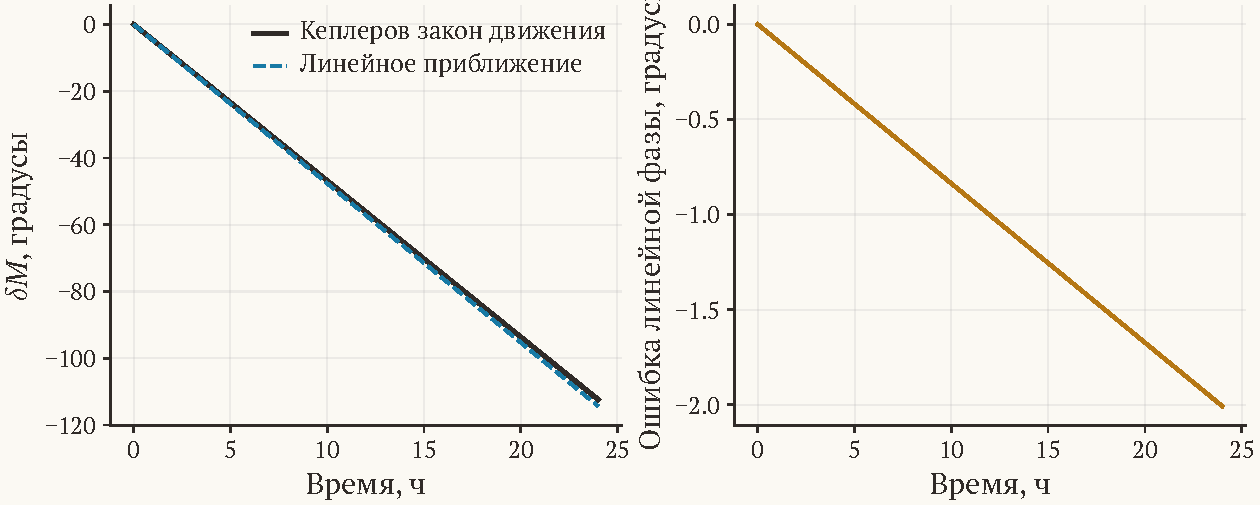
\includegraphics[width=\textwidth,height=56mm,keepaspectratio]{images/phi-phase-slide.pdf}\par}
$a=7000$ км, $\delta a=100$ км; интервал 24 ч.
\end{frame}

\begin{frame}{Импульсное изменение элементов}
\relax
\derivationmathspacing
\begin{columns}[T,onlytextwidth]
\begin{column}{.48\textwidth}
\textbf{Точный скачок скорости}
{\eqcompact\derivationmathspacing
\[
 \vect R_j^+=\vect R_j^-,\qquad
 \vect V_j^+=\vect V_j^-+Q_j\Delta\vect V_j,
\]
\[
 Q_j=[\vect e_{rj}\ \vect e_{tj}\ \vect e_{nj}].
\]
}
$\Delta\vect V_j$ задаётся в ОСК перед манёвром. Элементы после импульса вычисляются по новым $\vect R_j^+,\vect V_j^+$.
{\eqcompact\derivationmathspacing
\[
 \mathcal E^+-\mathcal E^-
 =\vect V^-\cdot Q_j\Delta\vect V_j
       +\frac12\|\Delta\vect V_j\|^2.
\]
}
\end{column}
\begin{column}{.49\textwidth}
\textbf{Первая производная по импульсу}
{\eqcompact\derivationmathspacing
\[
 \begin{aligned}
 \vect y_j^+-\vect y_j^-={}&B(\vect y_j^-)\Delta\vect V_j\\
 &+O(\|\Delta\vect V_j\|^2).
 \end{aligned}
\]
}
Положение непрерывно, но связь элементов со скоростью нелинейна. Матрица $B$ описывает только первый порядок.
\par\smallskip
Квадратичный член энергии показывает, почему линейное управление необходимо проверить точным скачком и нелинейным прогнозом.
\end{column}
\end{columns}
\end{frame}

\begin{frame}{Матрица манёвра}
\relax
\derivationmathspacing
{\eqcompact\derivationmathspacing
\[
 B_j=B(\vect y_0(t_j)),\qquad
 \delta\vect y(t_j^+)-\delta\vect y(t_j^-)=B_j\Delta\vect V_j.
\]
}
\begin{columns}[T,onlytextwidth]
\begin{column}{.46\textwidth}
\textbf{Перенос к конечному моменту}
{\eqcompact\derivationmathspacing
\[
 \delta\vect y_{f,j}=M_j\Delta\vect V_j,
\]
\[
 \boxed{M_j=\Phi(t_f,t_j)B(\vect y_0(t_j)).}
\]
}
$B_j$ задаёт мгновенное изменение элементов; $\Phi$ переносит его к $t_f$.

\end{column}
\begin{column}{.51\textwidth}
\textbf{Кеплерово движение}
{\eqcompact\derivationmathspacing
\[
 (M_j)_{1:5,:}=(B_j)_{1:5,:},
\]
\[
 (M_j)_{6,:}=(B_j)_{6,:}
     -\frac{3n}{2a}(t_f-t_j)(B_j)_{1,:}.
\]
}
Строка $M$ включает мгновенное изменение аномалии и накопленное изменение среднего движения.

\end{column}
\end{columns}
Матрица $M_j\in\mathbb R^{6\times3}$ связывает импульс с конечным изменением элементов.
\end{frame}

\begin{frame}{Линейная задача встречи}
\relax
\derivationmathspacing
Заданы моменты $t_i\le t_1<\ldots<t_N\le t_f$. Вклады импульсов складываются.
\begin{columns}[T,onlytextwidth]
\begin{column}{.55\textwidth}
{\eqcompact\derivationmathspacing
\[
 \sum_{j=1}^N M_j\Delta\vect V_j=\Delta\vect y_f.
\]
\[
 \Delta\vect V=
 \begin{pmatrix}\Delta\vect V_1\\\vdots\\\Delta\vect V_N\end{pmatrix}
 \in\mathbb R^{3N},
\]
\[
 \mathcal M=[M_1\ \cdots\ M_N]\in\mathbb R^{6\times3N},
\]
\[
 \boxed{\mathcal M\Delta\vect V=\Delta\vect y_f.}
\]
}
\end{column}
\begin{column}{.42\textwidth}
\textbf{Условия суперпозиции}
\begin{itemize}
\setlength{\itemsep}{4pt}
\item Блоки вычислены по одной $\vect y_0(t)$.
\item Изменения состояния и базисов следующих манёвров дают члены второго порядка.
\item Конечное состояние задаётся после всех импульсов.
\end{itemize}

\end{column}
\end{columns}
\end{frame}

\begin{frame}{Разрешимость и обусловленность}
\relax
\derivationmathspacing
\begin{columns}[T,onlytextwidth]
\begin{column}{.48\textwidth}
\textbf{Условие существования}
{\eqcompact\derivationmathspacing
\[
 \Delta\vect y_f\in\operatorname{Im}\mathcal M.
\]
}
\begin{itemize}
\setlength{\itemsep}{5pt}
\item $N=1$: ранг не выше трёх; произвольное шестимерное условие обычно недостижимо.
\item $N=2$: при $\det\mathcal M\ne0$ допустимое управление единственно.
\item $N>2$: возможно семейство решений, но полный ранг требует проверки.
\end{itemize}
\end{column}
\begin{column}{.49\textwidth}
\textbf{Масштабирование строк}
{\eqcompact\derivationmathspacing
\[
 \widehat{\mathcal M}=D_y^{-1}\mathcal M D_V,\qquad
 \Delta\widehat{\vect y}_f=D_y^{-1}\Delta\vect y_f.
\]
}
$D_y$ задаёт характерные масштабы элементов, $D_V$ --- скорости.
\par\smallskip
Близость столбцов к линейной зависимости усиливает чувствительность импульсов к исходным данным.
\par\smallskip
Число обусловленности немасштабированной матрицы зависит от единиц длины и углов.
\end{column}
\end{columns}
\end{frame}

\begin{frame}{Минимум характеристической скорости}
\relax
\derivationmathspacing
Моменты импульсов $t_j$ фиксированы.
\begin{columns}[T,onlytextwidth]
\begin{column}{.48\textwidth}
\textbf{Сумма норм импульсов}
{\eqcompact\derivationmathspacing
\[
 \begin{aligned}
 &\min_{\Delta\vect V}\ J=\sum_{j=1}^N\|\Delta\vect V_j\|,\\
 &\mathcal M\Delta\vect V=\Delta\vect y_f,\\
 &\|\Delta\vect V_j\|\le\Delta V_{\max,j}.
 \end{aligned}
\]
}
Сумма норм выпукла, равенство линейно. Вводя $s_j\ge0$, получаем ограничения $\|\Delta\vect V_j\|\le s_j$ и линейный критерий $\sum_j s_j$.
\end{column}
\begin{column}{.49\textwidth}
\textbf{Сумма квадратов норм}
{\eqcompact\derivationmathspacing
\[
 \min_{\Delta\vect V}\|\Delta\vect V\|^2,\quad
 \mathcal M\Delta\vect V=\Delta\vect y_f,
\]
\[
 \Delta\vect V_{\rm minnorm}
  =\mathcal M^\top(\mathcal M\mathcal M^\top)^{-1}
       \Delta\vect y_f.
\]
}
Формула справедлива при полном строчном ранге. На практике применяют QR- или сингулярное разложение.
\end{column}
\end{columns}
\smallskip
Минимумы суммы норм и суммы квадратов в общем случае различаются.
\end{frame}

\begin{frame}{Выбор моментов импульсов}
\relax
\derivationmathspacing
{\eqcompact\derivationmathspacing
\[
 \mathcal M=\mathcal M(t_1,\ldots,t_N),\qquad
 M_j=\Phi(t_f,t_j)B(\vect y_0(t_j)),
\]
}
\begin{columns}[T,onlytextwidth]
\begin{column}{.48\textwidth}
\textbf{Совместный выбор времён и импульсов}
\begin{itemize}
\setlength{\itemsep}{5pt}
\item $t_j$ входит в $B(\vect y_0(t_j))$ и длительность переноса до $t_f$.
\item Совместная задача становится нелинейной.
\item При выборе $t_f$ пересчитывается и $\Delta\vect y_f(t_f)$.
\end{itemize}
\end{column}
\begin{column}{.49\textwidth}
\textbf{Манёвры по аномалии или долготе}
\begin{itemize}
\setlength{\itemsep}{5pt}
\item Время достижения заданного угла зависит от управления.
\item В производных учитывается изменение времени события.
\item Найденное управление проверяется по исходной нелинейной динамике.
\end{itemize}
\end{column}
\end{columns}
\end{frame}

\begin{frame}{Функционал задачи встречи}
\relax
\derivationmathspacing
\begin{columns}[T,onlytextwidth]
\begin{column}{.56\textwidth}
\centering
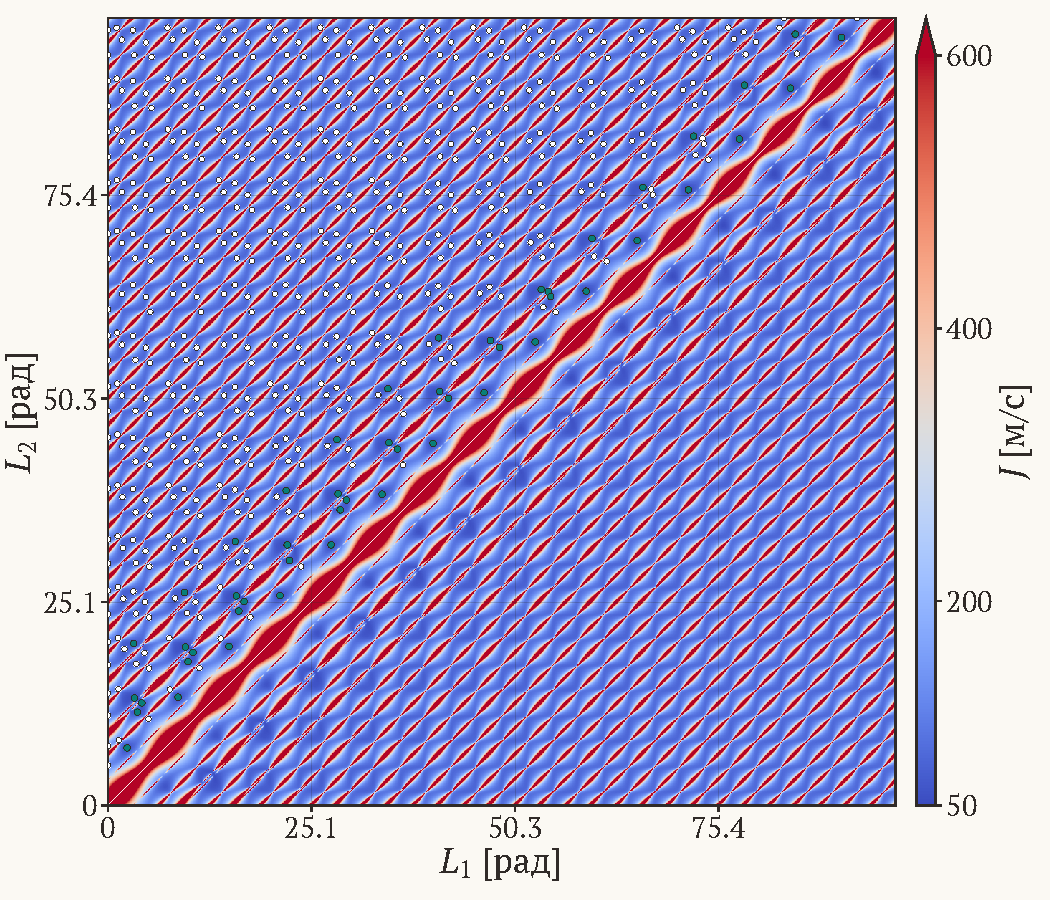
\includegraphics[width=\linewidth,height=62mm,keepaspectratio]{images/rendezvous-functional-slide.pdf}
\end{column}
\begin{column}{.41\textwidth}
Линейная встреча. $L_1,L_2$ --- развёрнутые долготы на $\vect y_0(t)$:
{\eqcompact\derivationmathspacing
\[
\begin{gathered}
 a=6800\ \text{км},\quad e=0{,}01,\quad i=45^\circ,\\
 \omega=\Omega=M_i=0,\\[2pt]
 \Delta\vect y_f=(1\ \text{км},\ 0{,}01,\ 1^\circ,\\[-2pt]
 \qquad0{,}1^\circ,\ 0{,}1^\circ,\ 1^\circ)^\top,\\[2pt]
 t_f-t_i=24\ \text{ч},\quad L=\Omega+\omega+\nu,\\
 0\le L_1,L_2\le97{,}2812\ \text{рад}.
\end{gathered}
\]
}
\begin{itemize}
\setlength{\itemsep}{0pt}
\item Белые точки --- найденные локальные минимумы.
\item Зелёные --- 50 лучших из найденных.
\end{itemize}
\end{column}
\end{columns}
\end{frame}


% Раздел Ламберта: обозначения и выводы из главы 3 методички rendezvous.tex.
% Вставляется между линейной встречей и моделью CW. Основной 7.tex не изменён.

\begin{frame}{Задача Ламберта}
\relax\derivationmathspacing
\begin{columns}[T,onlytextwidth]
\begin{column}{.50\textwidth}
\centering
\begin{tikzpicture}[course diagram,scale=.74]
\path[use as bounding box] (-5.5,-3.6) rectangle (2.8,3.8);
\def\pgeom{2.7115}
\def\egeom{.45}
\coordinate (O) at (0,0);
\coordinate (A) at ({\pgeom*cos(20)/(1+\egeom*cos(20))},
                    {\pgeom*sin(20)/(1+\egeom*cos(20))});
\coordinate (B) at ({\pgeom*cos(120)/(1+\egeom*cos(120))},
                    {\pgeom*sin(120)/(1+\egeom*cos(120))});
\draw[aux line] plot[domain=0:360,samples=100]
  ({\pgeom*cos(\x)/(1+\egeom*cos(\x))},
   {\pgeom*sin(\x)/(1+\egeom*cos(\x))});
\draw[orbit line,line width=1.4pt] plot[domain=20:120,samples=60]
  ({\pgeom*cos(\x)/(1+\egeom*cos(\x))},
   {\pgeom*sin(\x)/(1+\egeom*cos(\x))});
\draw[vector line] (O)--(A) node[pos=.54,below right] {$\vect R_1$};
\draw[vector line] (O)--(B) node[pos=.57,left] {$\vect R_2$};
\draw[courseaccent,dashed,line width=.8pt] (A)--(B);
\draw[angle line] (20:.85) arc[start angle=20,end angle=120,radius=.85]
  node[pos=.52,above right] {$\theta$};
\fill[courseink] (O) circle[radius=2.4pt];
\node[below left] at (O) {фокус};
\node[orbit point] at (A) {};
\node[right] at (A) {$1$};
\node[orbit point] at (B) {};
\node[above left] at (B) {$2$};
\end{tikzpicture}

\par
\figcaption{Два радиус-вектора и ориентированный угол $\theta$.}
\end{column}
\begin{column}{.46\textwidth}
Дано: $\vect R_1,\vect R_2$, $\tau=t_2-t_1>0$, $\mu$.
\par\smallskip
Найти $\vect V_1,\vect V_2$ на кеплеровой дуге:
{\eqcompact\derivationmathspacing
\[
 \ddot{\vect R}=-\frac{\mu}{R^3}\vect R,
 \qquad R_j=\|\vect R_j\|,
\]
\[
 \vect R(t_1)=\vect R_1,\qquad
 \vect R(t_2)=\vect R_2.
\]
}
\justifying
Заданы направление обхода и $m$ полных оборотов.
Знак нормали выбирает $0<\theta<\pi$ или $\pi<\theta<2\pi$.
\par\smallskip
При $\sin\theta=0$ нужны отдельный выбор плоскости и предельные формулы.
\end{column}
\end{columns}
\end{frame}

\begin{frame}{Два положения и семейство коник}
\relax\derivationmathspacing
{\eqcompact\derivationmathspacing
\[
 \vect e_1=\frac{\vect R_1}{R_1},\qquad
 \vect e_3=\pm\frac{\vect R_1\times\vect R_2}{\|\vect R_1\times\vect R_2\|},
 \qquad \vect e_2=\vect e_3\times\vect e_1.
\]
}
\begin{columns}[T,onlytextwidth]
\begin{column}{.48\textwidth}
{\eqcompact\derivationmathspacing
\[
 \frac{\vect R_2}{R_2}
 =\cos\theta\,\vect e_1+\sin\theta\,\vect e_2,
\]
\[
 \vect e=e_c\vect e_1+e_s\vect e_2,
 \qquad R(\eta)=\frac p{D(\eta;p)},
\]
\[
 D(\eta;p)=1+e_c\cos\eta+e_s\sin\eta.
\]
}
\justifying
Угол $\eta$ отсчитывается от $\vect R_1$; истинная аномалия $\nu=\eta-\varpi$.
\end{column}
\begin{column}{.48\textwidth}
{\eqcompact\derivationmathspacing
\[
 1+e_c=\frac p{R_1},\qquad
 1+e_c\cos\theta+e_s\sin\theta=\frac p{R_2},
\]
\[
 \boxed{\begin{aligned}
 e_c(p)&=\frac p{R_1}-1,\\[4pt]
 e_s(p)&=\frac{p/R_2-1-e_c(p)\cos\theta}{\sin\theta}.
 \end{aligned}}
\]
\[
 e=\sqrt{e_c^2+e_s^2},\qquad
 \varpi=\operatorname{atan2}(e_s,e_c).
\]
}
\end{column}
\end{columns}
\end{frame}

\begin{frame}{Параметр $p$: форма коники и время}
\relax\derivationmathspacing
\begin{columns}[T,onlytextwidth]
\begin{column}{.75\textwidth}
\centering
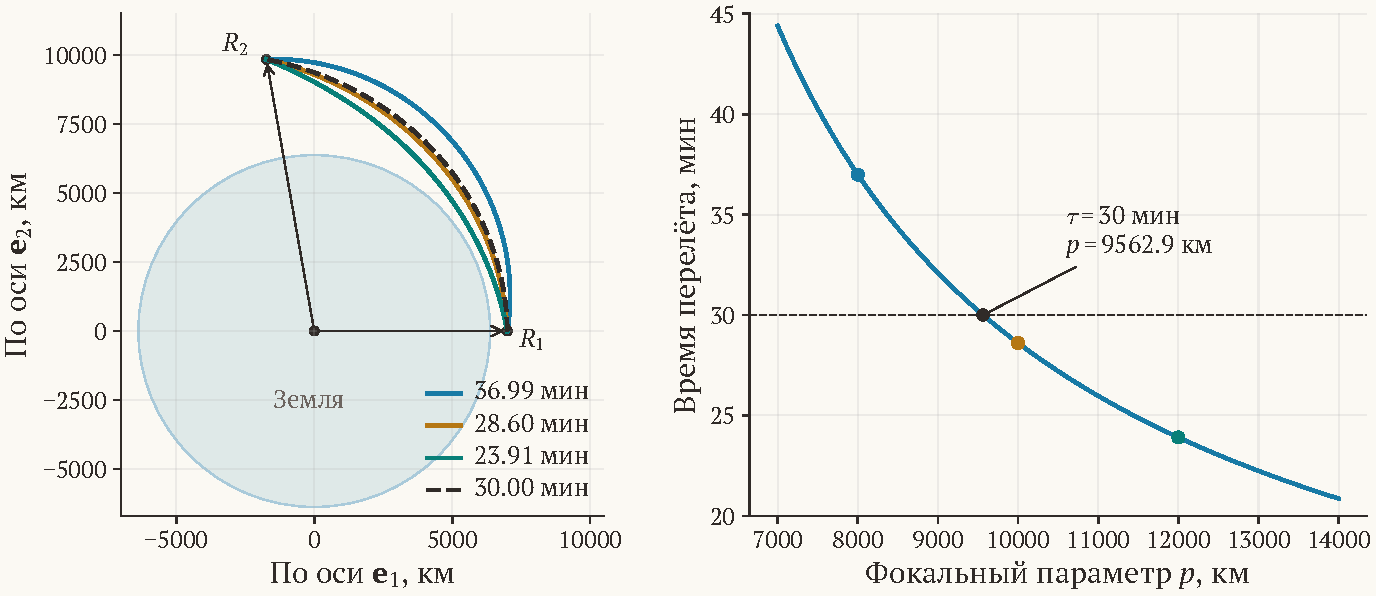
\includegraphics[width=\linewidth,height=55mm,keepaspectratio]{images/lambert-family-slide.pdf}
\par
\figcaption{$R_1=7000$ км, $R_2=10000$ км, $\theta=100^\circ$.
Три значения $p$ дают разные дуги и времена; выделено решение для $\tau=30$ мин.}
\end{column}
\begin{column}{.22\textwidth}
При $e\ne1$:
{\eqcompact\derivationmathspacing
\[
 a(p)=\frac p{1-e(p)^2}.
\]
\setlength{\arraycolsep}{2pt}
\[
 \begin{array}{ll}
 e<1:&\text{эллипс},\\[4pt]
 e=1:&\text{парабола},\\[4pt]
 e>1:&\text{гипербола}.
 \end{array}
\]
}
\justifying
При $e<1$ имеем $a>0$, при $e>1$ --- $a<0$.
\end{column}
\end{columns}
\end{frame}

\begin{frame}{От закона площадей к времени перелёта}
\relax\derivationmathspacing
\begin{columns}[T,onlytextwidth]
\begin{column}{.40\textwidth}
Сохраняется удельный момент:
{\eqcompact\derivationmathspacing
\[
 R^2\dot\eta=h=\sqrt{\mu p},
 \qquad \mathrm dt=\frac{R^2}{\sqrt{\mu p}}\,\mathrm d\eta.
\]
}
\justifying
На всей выбранной дуге:
{\eqcompact\derivationmathspacing
\[
 p>0,\qquad D(\eta;p)>0,
\]
\[
 0\le\eta\le\theta+2\pi m.
\]
}
Для эллипса $D>0$ при любом $\eta$; только эллипс допускает $m>0$.
\par\smallskip
Проверяем $R>R_{\min}$ по концам и перицентрам дуги.
\end{column}
\begin{column}{.56\textwidth}
Интегрируем вдоль дуги:
{\eqcompact\derivationmathspacing
\[
 \begin{aligned}
 T_m(p)&=\frac1{\sqrt{\mu p}}
  \int_0^{\theta+2\pi m}R(\eta;p)^2\,\mathrm d\eta\\[5pt]
 &=\frac{p^{3/2}}{\sqrt\mu}
  \int_0^{\theta+2\pi m}\frac{\mathrm d\eta}{D(\eta;p)^2}.
 \end{aligned}
\]
\[
 \boxed{F_m(p)=T_m(p)-\tau=0.}
\]
}
\justifying
После определения $e_c(p),e_s(p)$ остаётся одно скалярное условие времени.
\par\smallskip
При $m=0$ и невырожденной геометрии заданное время определяет одну дугу для выбранного направления.
\end{column}
\end{columns}
\end{frame}

\begin{frame}{Время перелёта по эллипсу}
\relax\derivationmathspacing
Аномалии концов определяются ориентацией найденной коники:
{\eqcompact\derivationmathspacing
\[
 \nu_1=-\varpi,\qquad \nu_2=\theta-\varpi+2\pi m.
\]
}
\begin{columns}[T,onlytextwidth]
\begin{column}{.46\textwidth}
Переход к эксцентрической аномалии:
{\eqcompact\derivationmathspacing
\[
 \begin{aligned}
 \cos E&=\frac{e+\cos\nu}{1+e\cos\nu},\\[4pt]
 \sin E&=\frac{\sqrt{1-e^2}\sin\nu}{1+e\cos\nu}.
 \end{aligned}
\]
\[
 n\,\mathrm dt=(1-e\cos E)\,\mathrm dE.
\]
}
\end{column}
\begin{column}{.50\textwidth}
Интегрирование даёт время:
{\eqcompact\derivationmathspacing
\[
 nT_m=\int_{E_1}^{E_2}(1-e\cos E)\,\mathrm dE,
\]
\[
 \boxed{\begin{aligned}
 T_m=\sqrt{\frac{a^3}{\mu}}\bigl[&E_2-E_1\\[-1pt]
 &-e(\sin E_2-\sin E_1)\bigr].
 \end{aligned}}
\]
}
\end{column}
\end{columns}
\smallskip
\justifying
$E_1,E_2$ непрерывно продолжаются вдоль дуги с учётом $m$.
Сведение по модулю $2\pi$ перед вычитанием теряет полные периоды.
\end{frame}

\begin{frame}{Гипербола и параболический предел}
\relax\derivationmathspacing
\begin{columns}[T,onlytextwidth]
\begin{column}{.48\textwidth}
Для гиперболы $e>1$, $a=p/(1-e^2)<0$:
{\eqcompact\derivationmathspacing
\[
 \sinh H=\frac{\sqrt{e^2-1}\sin\nu}{1+e\cos\nu},
\]
\[
 \begin{aligned}
 T=\sqrt{\frac{(-a)^3}{\mu}}\bigl[&e(\sinh H_2-\sinh H_1)\\[-1pt]
 &-(H_2-H_1)\bigr].
 \end{aligned}
\]
}
\justifying
Знаменатель $1+e\cos\nu$ должен оставаться положительным на всей дуге: пересекать асимптоту нельзя.
\end{column}
\begin{column}{.48\textwidth}
Для параболы $e=1$ --- формула Баркера:
{\eqcompact\derivationmathspacing
\[
 D_B=\tan\frac\nu2,
\]
\[
 \begin{aligned}
 T=\frac12\sqrt{\frac{p^3}{\mu}}\Bigl[&D_{B2}+\frac{D_{B2}^3}{3}\\[-1pt]
 &-D_{B1}-\frac{D_{B1}^3}{3}\Bigr].
 \end{aligned}
\]
}
\justifying
Здесь $\nu_1=-\varpi$, $\nu_2=\theta-\varpi$; полных оборотов нет, $m=0$.
\end{column}
\end{columns}
\smallskip
\justifying
При $e\to1$ величина $a$ растёт по модулю; выражения через $a$ и аномалии могут вычитать большие близкие величины.
Угловой интеграл $T_m(p)$ сохраняет смысл и в параболическом пределе.
\end{frame}

\begin{frame}{Ветви решения Ламберта}
\relax\derivationmathspacing
\begin{columns}[T,onlytextwidth]
\begin{column}{.72\textwidth}
\centering
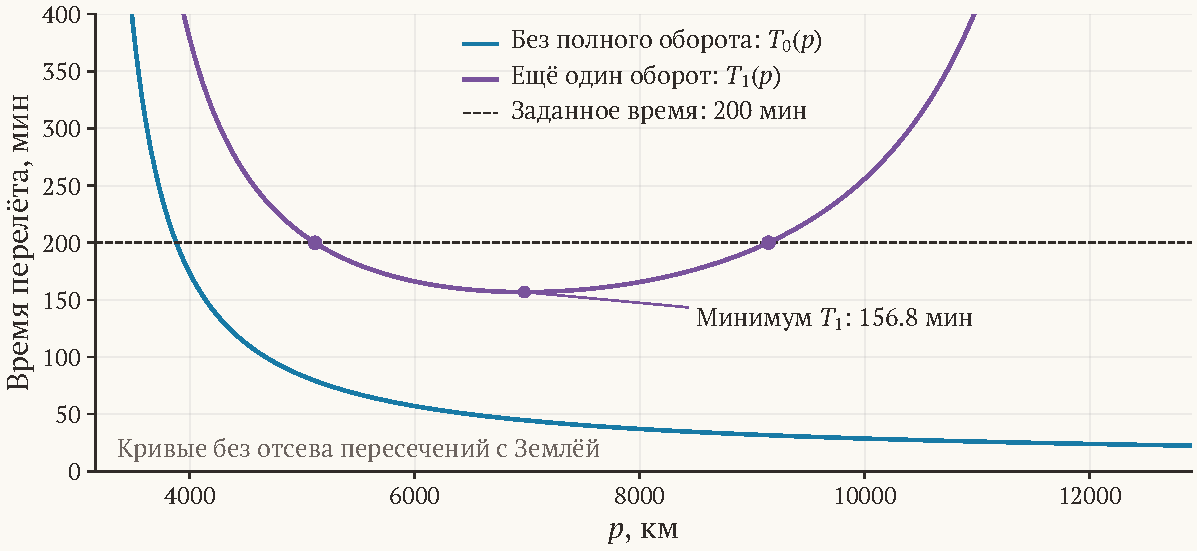
\includegraphics[width=\linewidth,height=54mm,keepaspectratio]{images/lambert-branches-slide.pdf}
\par
\figcaption{$R_1=7000$ км, $R_2=10000$ км, $\theta=100^\circ$.
Дуги, пересекающие Землю, при построении не исключены.}
\end{column}
\begin{column}{.25\textwidth}
Без дополнительных ограничений ($m\ge1$):
{\eqcompact\derivationmathspacing
\[
 \begin{array}{ll}
 \tau<T_{m,\min}:&0,\\[4pt]
 \tau=T_{m,\min}:&1,\\[4pt]
 \tau>T_{m,\min}:&2.
 \end{array}
\]
}
На рисунке $T_{1,\min}\simeq156{,}8$ мин.
При $\tau=200$ мин:
{\eqcompact\derivationmathspacing
\[
 \begin{aligned}
 p&\simeq5112{,}9\ \text{км},\\
 p&\simeq9145{,}0\ \text{км}.
 \end{aligned}
\]
}
\end{column}
\end{columns}
\end{frame}

\begin{frame}{Поиск корня на выбранной ветви}
\relax\derivationmathspacing
\begin{columns}[T,onlytextwidth]
\begin{column}{.39\textwidth}
\begin{enumerate}
\setlength{\itemsep}{3pt}
\item Задать направление, $m$ и допустимый интервал $p$.
\item Вычислить $e_c,e_s,e,T_m$.
\item Для каждой ветви найти смену знака $F_m$.
\item Бисекция или Ньютон внутри интервала.
\end{enumerate}
{\eqcompact\derivationmathspacing
\[
 p\ \leftarrow\ p-\frac{F_m(p)}{\mathrm dT_m/\mathrm dp}.
\]
}
\end{column}
\begin{column}{.57\textwidth}
Производная из углового интеграла:
{\eqcompact\derivationmathspacing
\[
 \begin{aligned}
 \frac{\mathrm dT_m}{\mathrm dp}
 &=\frac{3T_m}{2p}
 -\frac{2p^{3/2}}{\sqrt\mu}\times\\[3pt]
 &\quad\int_0^{\theta+2\pi m}
 \frac{D_p(\eta;p)}{D(\eta;p)^3}\,\mathrm d\eta,
 \end{aligned}
\]
\[
 \begin{aligned}
 D_p(\eta;p)&=\frac{\cos\eta}{R_1}\\[3pt]
 &+\frac{1/R_2-\cos\theta/R_1}{\sin\theta}\sin\eta.
 \end{aligned}
\]
}
\justifying
Производная определена внутри допустимого интервала.
В минимуме ветви проверяют касательный корень: знак $F_m$ не меняется.
\end{column}
\end{columns}
\end{frame}

\begin{frame}{Восстановление скоростей через $f,g$}
\relax\derivationmathspacing
Для найденного $p$:
{\eqcompact\derivationmathspacing
\[
 f=1-\frac{R_2}{p}(1-\cos\theta),\qquad
 g=\frac{R_1R_2\sin\theta}{\sqrt{\mu p}},\qquad
 \dot g=1-\frac{R_1}{p}(1-\cos\theta).
\]
}
\begin{columns}[T,onlytextwidth]
\begin{column}{.46\textwidth}
Связь положений и скоростей:
{\eqcompact\derivationmathspacing
\[
 \vect R_2=f\vect R_1+g\vect V_1,
\]
\[
 \vect V_2=\dot f\vect R_1+\dot g\vect V_1,
 \qquad f\dot g-\dot f g=1.
\]
\[
 \begin{aligned}
 \vect V_2&=\frac{\dot g}{g}\vect R_2
 +\left(\dot f-\frac{f\dot g}{g}\right)\vect R_1\\[3pt]
 &=\frac{\dot g}{g}\vect R_2-\frac1g\vect R_1.
 \end{aligned}
\]
}
\end{column}
\begin{column}{.50\textwidth}
Скорости получаются алгебраически:
{\eqcompact\derivationmathspacing
\[
 \boxed{\vect V_1=\frac{\vect R_2-f\vect R_1}{g},\qquad
 \vect V_2=\frac{\dot g\vect R_2-\vect R_1}{g}.}
\]
}
Геометрическая проверка компонент:
{\eqcompact\derivationmathspacing
\[
 V_r=\sqrt{\frac\mu p}(e_c\sin\eta-e_s\cos\eta),
 \qquad V_t=\frac{\sqrt{\mu p}}{R(\eta)}.
\]
}
\end{column}
\end{columns}
\smallskip
\justifying
При $\theta\to0$ или $\pi$ коэффициент $g$ мал.
Строго коллинеарные концы требуют дополнительного выбора плоскости и предельных формул.
\end{frame}

\begin{frame}{Дуга Ламберта в задаче встречи}
\relax\derivationmathspacing
\justifying
При импульсах в $t_i,t_f$ первый конец дуги --- начальное положение управляемого КА,
второй --- положение цели в $t_f$. Найденные $\vect V_1,\vect V_2$ заданы в инерциальных осях.
\begin{columns}[T,onlytextwidth]
\begin{column}{.48\textwidth}
Импульсы в инерциальных осях:
{\eqcompact\derivationmathspacing
\[
 \boxed{\begin{aligned}
 \Delta\vect V_{1,I}&=\vect V_1-\vect V_C(t_i^-),\\[4pt]
 \Delta\vect V_{2,I}&=\vect V_{\rm tar}(t_f)-\vect V_2.
 \end{aligned}}
\]
}
\justifying
Нелинейное конечное условие выполнено в центральном поле для выбранных времени и ветви.
При возмущениях это начальное приближение.
\end{column}
\begin{column}{.48\textwidth}
Проекция в предманёвренные ОСК:
{\eqcompact\derivationmathspacing
\[
 \Delta\vect V_j=Q_j^\top\Delta\vect V_{j,I},
\]
\[
 Q_j=[\vect e_{rj}\ \vect e_{tj}\ \vect e_{nj}],
\]
\[
 J=\|\Delta\vect V_1\|+\|\Delta\vect V_2\|.
\]
}
\justifying
Каждый $Q_j$ задан состоянием до импульса.
Для второго используется конец пассивной дуги.
\end{column}
\end{columns}
\smallskip
Поиск минимума $J$ по временам --- отдельная задача;
решение Ламберта относится к уже выбранным времени и ветви.
\end{frame}


% Относительное движение: обозначения и последовательность глав 4--6 методички.
\begin{frame}{Относительные координаты}
\relax
\derivationmathspacing
Для кеплеровой цели $\vect R_0(t),\vect V_0(t)$ --- инерциальные положение и скорость;
$Q_0=(\vect e_r\ \vect e_t\ \vect e_n)$ --- её базис RTN.
{\eqcompact\derivationmathspacing
\[
 \vect\rho=Q_0^\top(\vect R_C-\vect R_0)=(x,y,z)^\top,
 \qquad \vect\Omega_r=(0,0,\omega_r)^\top,\qquad
 \omega_r=\dot\nu_0=\frac{h_0}{R_0^2}.
\]
\[
 Q_0^\top(\vect V_C-\vect V_0)
 =\dot{\vect\rho}+\vect\Omega_r\times\vect\rho,
 \quad
 \begin{aligned}
 \delta V_r&=\dot x-\omega_r y,\\
 \delta V_t&=\dot y+\omega_r x,\quad \delta V_n=\dot z.
 \end{aligned}
\]
\[
\begin{aligned}
 Q_0^\top(\ddot{\vect R}_C-\ddot{\vect R}_0)
 ={}&\ddot{\vect\rho}+2\vect\Omega_r\times\dot{\vect\rho}
 +\dot{\vect\Omega}_r\times\vect\rho\\[-1pt]
 &+\vect\Omega_r\times(\vect\Omega_r\times\vect\rho).
\end{aligned}
\]
}
\justifying
Ось $x$ радиальна, $y$ поперечна радиусу, $z$ нормальна плоскости.
Производные координат отличаются от проекций разности инерциальных скоростей.
{\eqcompact\derivationmathspacing
\[
 \vect R_{Ci}=\vect R_{0i}+Q_{0i}\vect\rho_i,\qquad
 \vect V_{Ci}=\vect V_{0i}
 +Q_{0i}(\dot{\vect\rho}_i+\vect\Omega_{ri}\times\vect\rho_i).
\]
}
\end{frame}

\begin{frame}{Точные относительные уравнения}
\relax
\derivationmathspacing
Центральное поле; $\vect u$ --- разность добавочных ускорений в RTN цели.
{\eqcompact\derivationmathspacing
\[
\begin{aligned}
 \ddot{\vect\rho}={}&-\mu\left[
 \frac{R_0\vect e_x+\vect\rho}
 {\lVert R_0\vect e_x+\vect\rho\rVert^3}
 -\frac{\vect e_x}{R_0^2}\right]
 -2\vect\Omega_r\times\dot{\vect\rho}
 -\dot{\vect\Omega}_r\times\vect\rho\\[-1pt]
 &-\vect\Omega_r\times(\vect\Omega_r\times\vect\rho)+\vect u,
 \qquad \vect e_x=(1,0,0)^\top.
\end{aligned}
\]
\[
 d=\sqrt{(R_0+x)^2+y^2+z^2},\qquad
 \boxed{\begin{aligned}
 \ddot x-2\omega_r\dot y-\dot\omega_r y-\omega_r^2x
 &=-\frac{\mu(R_0+x)}{d^3}+\frac{\mu}{R_0^2}+u_x,\\[4pt]
 \ddot y+2\omega_r\dot x+\dot\omega_r x-\omega_r^2y
 &=-\frac{\mu y}{d^3}+u_y,\\[4pt]
 \ddot z&=-\frac{\mu z}{d^3}+u_z.
 \end{aligned}}
\]
}
\justifying
При пассивной цели $\vect u$ --- управляющее ускорение аппарата в RTN цели.
\end{frame}

\begin{frame}{Линеаризация: модель CW}
\relax
\derivationmathspacing
Круговая кеплерова цель: $R_0=a_0$, $\omega_r=n_0=\sqrt{\mu/a_0^3}$,
$\dot\omega_r=0$. При $\lVert\vect\rho\rVert/a_0\ll1$:
{\eqcompact\derivationmathspacing
\[
 -\mu\left[
 \frac{a_0\vect e_x+\vect\rho}{\lVert a_0\vect e_x+\vect\rho\rVert^3}
 -\frac{\vect e_x}{a_0^2}\right]
 =n_0^2(2x,-y,-z)^\top
 +O\!\left(\frac{\mu\lVert\vect\rho\rVert^2}{a_0^4}\right).
\]
}
\begin{columns}[T,onlytextwidth]
\begin{column}{.48\textwidth}
Радиальная строка точной системы:
{\eqcompact\derivationmathspacing
\[
 \ddot x-2n_0\dot y-n_0^2x=2n_0^2x+u_x.
\]
}
\justifying
Сумма радиального гравитационного градиента и центробежного члена даёт коэффициент $3n_0^2$.
\end{column}
\begin{column}{.48\textwidth}
{\eqcompact\derivationmathspacing
\[
 \boxed{\begin{aligned}
 \ddot x-2n_0\dot y-3n_0^2x&=u_x,\\[4pt]
 \ddot y+2n_0\dot x&=u_y,\\[4pt]
 \ddot z+n_0^2z&=u_z.
 \end{aligned}}
\]
}
\end{column}
\end{columns}
\smallskip
\justifying
Уравнения Клохесси--Уилтшира (CW) сохраняют первый порядок по относительному расстоянию.
Декартовы координаты RTN определены при $e=0$, хотя классические элементы при этом вырождены.
\end{frame}

\begin{frame}{Свободное движение и дрейф}
\relax
\derivationmathspacing
При $\vect u=0$ интегрируем вторую строку CW и подставляем результат в первую:
{\eqcompact\derivationmathspacing
\[
 \dot y+2n_0x=C,\qquad C=\dot y_i+2n_0x_i,
 \qquad \boxed{\ddot x+n_0^2x=2n_0C.}
\]
}
\begin{columns}[T,onlytextwidth]
\begin{column}{.56\textwidth}
Начало времени совмещено с $t_i$:
{\eqcompact\derivationmathspacing
\[
\begin{aligned}
 x&=A\cos(n_0t)+B\sin(n_0t)+\frac{2C}{n_0},\\[4pt]
 y&=-2A\sin(n_0t)+2B\cos(n_0t)-3Ct+D,\\[4pt]
 z&=E\cos(n_0t)+F\sin(n_0t).
\end{aligned}
\]
}
$A,B,C,D,E,F$ --- постоянные решения.
\end{column}
\begin{column}{.40\textwidth}
{\eqcompact\derivationmathspacing
\[
 x_c=\frac{2C}{n_0},\qquad
 \dot y_{\rm secular}=-\frac32n_0x_c,
\]
\[
 C=0\ \Longleftrightarrow\ \dot y_i=-2n_0x_i.
\]
}
\justifying
$C$ задаёт смещение центра и дрейф. При $x_c>0$ аппарат в среднем отстаёт от цели.
Нулевое $\dot{\vect\rho}_i$ само по себе дрейф не устраняет.
\end{column}
\end{columns}
\end{frame}

\begin{frame}{Решение CW через начальное состояние}
\relax
\derivationmathspacing
Определяя постоянные по $x_i,y_i,z_i,\dot x_i,\dot y_i,\dot z_i$, получаем
($c=\cos n_0t$, $s=\sin n_0t$):
\begin{columns}[T,onlytextwidth]
\begin{column}{.59\textwidth}
{\eqcompact\derivationmathspacing
\[
\begin{aligned}
 x&=(4-3c)x_i+\frac{s}{n_0}\dot x_i
                    +\frac{2(1-c)}{n_0}\dot y_i,\\[5pt]
 y&=6(s-n_0t)x_i+y_i-\frac{2(1-c)}{n_0}\dot x_i\\[-1pt]
  &\hspace{23mm}+\frac{4s-3n_0t}{n_0}\dot y_i,\\[5pt]
 z&=cz_i+\frac{s}{n_0}\dot z_i.
\end{aligned}
\]
}
\end{column}
\begin{column}{.37\textwidth}
{\eqcompact\derivationmathspacing
\[
\begin{aligned}
 \dot x&=3n_0sx_i+c\dot x_i+2s\dot y_i,\\[5pt]
 \dot y&=6n_0(c-1)x_i-2s\dot x_i\\[-1pt]
       &\hspace{14mm}+(4c-3)\dot y_i,\\[5pt]
 \dot z&=-n_0sz_i+c\dot z_i.
\end{aligned}
\]
}
\end{column}
\end{columns}
\justifying
Коэффициенты образуют $\Phi_{\rm CW}(t,t_i)$ для
$\vect X=(x,y,z,\dot x,\dot y,\dot z)^\top$.
Условие $\vect X_f=0$ означает совпадение положения и инерциальной скорости.
\end{frame}

\begin{frame}{Плоское относительное движение}
\relax
\derivationmathspacing
{\eqcompact\derivationmathspacing
\[
 a_0=7000\ \text{км},\quad x_i=100\ \text{м},\quad y_i=\dot x_i=0,
 \qquad \dot y_i=-2n_0x_i\ \text{или}\ -1{,}7n_0x_i.
\]
}
\centering
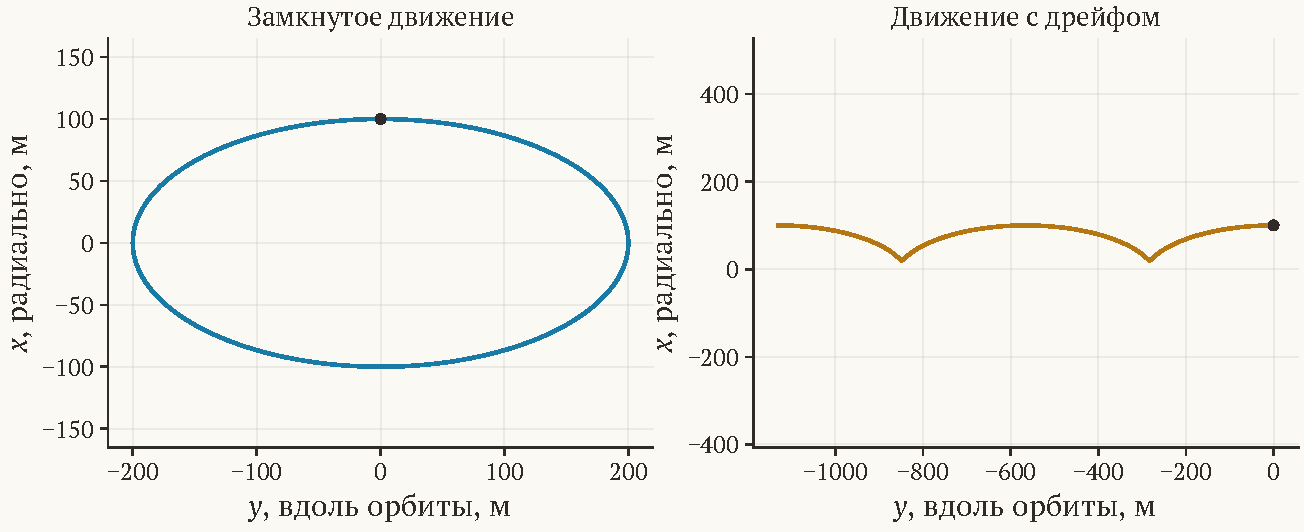
\includegraphics[width=.98\linewidth,height=44mm,keepaspectratio]{images/cw-modes-slide.pdf}
\par
\justifying
Слева $C=0$: эллипс $2:1$. Справа $C\ne0$: смещение центра $x_c=2C/n_0$ и дрейф $-3Ct$.
\end{frame}

\begin{frame}{Пространственное движение CW}
\relax
\derivationmathspacing
\centering
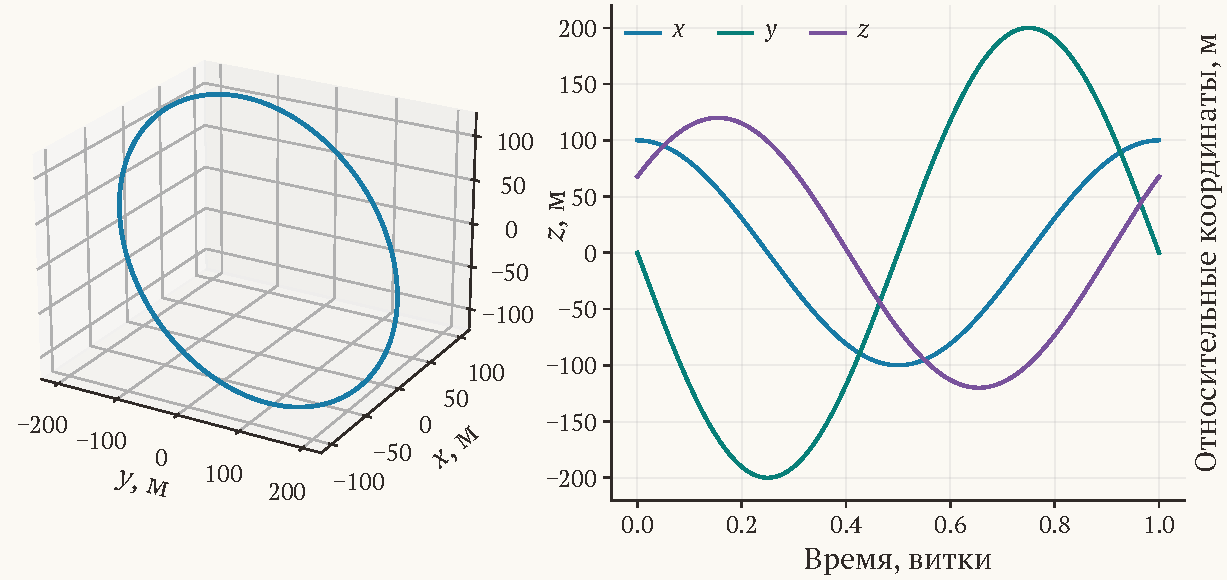
\includegraphics[width=.98\linewidth,height=43.5mm,keepaspectratio]{images/cw-spatial-slide.pdf}
\par
{\eqcompact\derivationmathspacing
\[
 x=100\cos n_0t,\qquad y=-200\sin n_0t,\qquad
 z=120\sin(n_0t+0{,}6)\quad\text{(координаты в метрах).}
\]
}
\justifying
Общая частота и отсутствие дрейфа дают эллипс в пространстве. Фаза нормального колебания меняет его ориентацию.
\end{frame}

\begin{frame}{Эллиптическая орбита: система TH}
\relax
\derivationmathspacing
{\eqcompact\derivationmathspacing
\[
 R_0=\frac{p_0}{1+e_0\cos\nu_0},\qquad
 \omega_r=\frac{h_0}{R_0^2},\qquad
 \dot\omega_r=-2\frac{\dot R_0}{R_0}\omega_r.
\]
\[
 -\mu\left[
 \frac{R_0\vect e_x+\vect\rho}{\lVert R_0\vect e_x+\vect\rho\rVert^3}
 -\frac{\vect e_x}{R_0^2}\right]
 \simeq\frac{\mu}{R_0^3}(2x,-y,-z)^\top.
\]
\[
 \boxed{\begin{aligned}
 \ddot x&=\left(\omega_r^2+2\mu/R_0^3\right)x
              +2\omega_r\dot y+\dot\omega_r y+u_x,\\[4pt]
 \ddot y&=\left(\omega_r^2-\mu/R_0^3\right)y
              -2\omega_r\dot x-\dot\omega_r x+u_y,\\[4pt]
 \ddot z&=-\mu z/R_0^3+u_z.
 \end{aligned}}
\]
}
\justifying
В TH сохраняются переменные $R_0,\omega_r$ и полная зависимость от $e_0$.
При $e_0\to0$: $\omega_r^2=\mu/R_0^3=n_0^2$, $\dot\omega_r=0$; получается CW.
\end{frame}

\begin{frame}{Решение Яманаки--Анкерсена}
\relax
\derivationmathspacing
\begin{columns}[T,onlytextwidth]
\begin{column}{.47\textwidth}
Для пассивной системы $\vect u=0$:
{\eqcompact\derivationmathspacing
\[
 \sigma=1+e_0\cos\nu_0,\qquad
 \widetilde{\vect\rho}=\sigma\vect\rho,
\]
\[
 \frac{\mathrm d}{\mathrm dt}=\omega_r\frac{\mathrm d}{\mathrm d\nu_0},
 \qquad \ddot x=\omega_r^2x''+\dot\omega_r x',
\]
\[
 \begin{aligned}
 \widetilde x''-2\widetilde y'-\frac3\sigma\widetilde x&=0,\\[4pt]
 \widetilde y''+2\widetilde x'&=0,\\[4pt]
 \widetilde z''+\widetilde z&=0.
 \end{aligned}
\]
}
Штрих --- производная по $\nu_0$.
\end{column}
\begin{column}{.49\textwidth}
{\eqcompact\derivationmathspacing
\[
 \vect X=(\vect\rho,\dot{\vect\rho})^\top,\quad
 \widetilde{\vect X}=
 \begin{pmatrix}\widetilde{\vect\rho}\\\widetilde{\vect\rho}'\end{pmatrix}
 =\mathcal T\vect X,
\]
\[
 \mathcal T=
 \begin{pmatrix}
 \sigma I_3&0\\[3pt]
 \sigma'I_3&(\sigma/\omega_r)I_3
 \end{pmatrix},
\]
\[
 \begin{aligned}
 \Phi_{\rm TH}(t,t_i)
 &=\mathcal T(\nu_0)^{-1}Y(\nu_0)\\[-1pt]
 &\quad\times Y(\nu_i)^{-1}\mathcal T(\nu_i).
 \end{aligned}
\]
}
$Y$ --- фундаментальная матрица; YA регулярно при $e_0=0$.
\end{column}
\end{columns}
{\eqcompact\derivationmathspacing
\[
 \mathcal J(\nu_0,\nu_i)
 =\int_{\nu_i}^{\nu_0}\frac{\mathrm d\eta}{(1+e_0\cos\eta)^2}
 =\sqrt{\frac\mu{p_0^3}}(t-t_i),\qquad 0\le e_0<1.
\]
}
\end{frame}

\begin{frame}{Сравнение CW и TH}
\relax
\derivationmathspacing
{\eqcompact\derivationmathspacing
\[
 a_0=10000\ \text{км},\quad e_0=0{,}2,\quad\nu_i=0,\qquad
 \vect\rho_i=(0,-100,10)^\top\ \text{м},\quad
 \dot{\vect\rho}_i=0.
\]
}
\centering
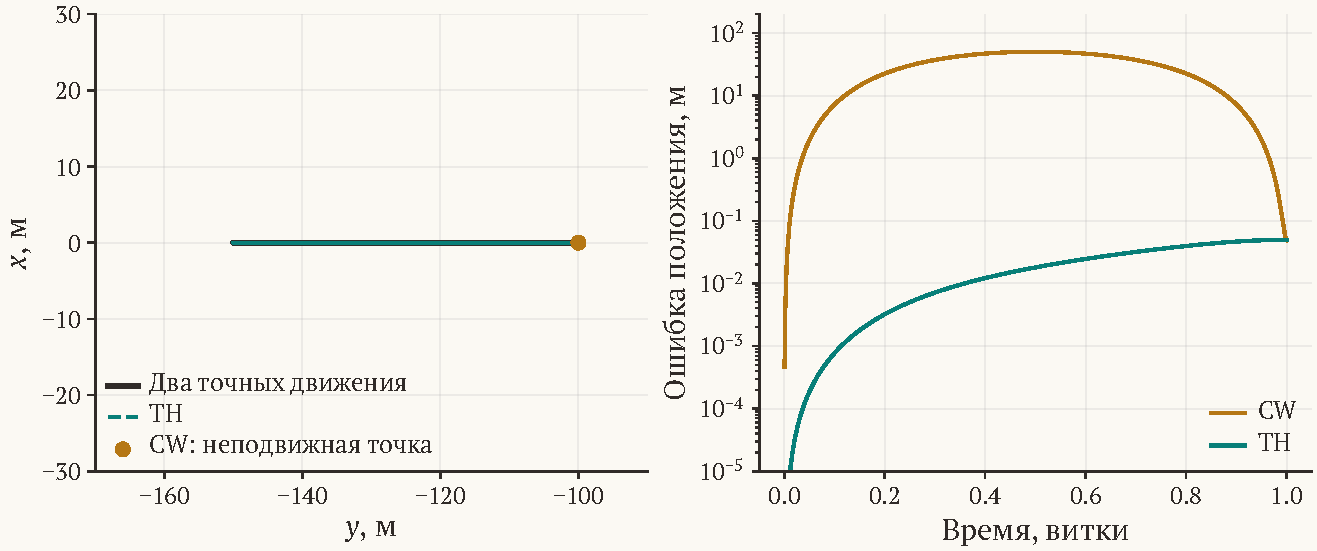
\includegraphics[width=.98\linewidth,height=42.5mm,keepaspectratio]{images/relative-elliptic-slide.pdf}
\par
\justifying
CW: $n_0=\sqrt{\mu/a_0^3}$. Максимальные ошибки: $50{,}27$ м (CW), $0{,}050$ м (TH); конечные --- около $0{,}050$ м у обеих моделей.
\end{frame}

\begin{frame}{Усреднение и опорная орбита с $J_2$}
\relax
\derivationmathspacing
$R_E$ --- экваториальный радиус Земли; $J_2$ --- вторая зональная гармоника.
\begin{columns}[T,onlytextwidth]
\begin{column}{.48\textwidth}
В инерциальных экваториальных осях:
{\eqcompact\derivationmathspacing
\[
 \vect a_{J_2}=\frac{3J_2\mu R_E^2}{2R^5}
 \begin{pmatrix}
 X(5Z^2/R^2-1)\\[2pt]
 Y(5Z^2/R^2-1)\\[2pt]
 Z(5Z^2/R^2-3)
 \end{pmatrix}.
\]
\[
 \dot{\overline\Omega}
 =-\frac32J_2n\left(\frac{R_E}{p}\right)^2\cos i.
\]
}
\justifying
Черта --- усреднение. Оскулирующие элементы имеют также короткопериодические изменения.
\end{column}
\begin{column}{.48\textwidth}
Опорная орбита SS имеет радиус $r_{\rm ref}$ и наклонение $i_{\rm ref}$:
{\eqcompact\derivationmathspacing
\[
 s=\frac{3J_2R_E^2}{8r_{\rm ref}^2}(1+3\cos2i_{\rm ref}),
\]
\[
 c=\sqrt{1+s},\qquad n=\sqrt{\mu/r_{\rm ref}^3},
\]
\[
 \left\langle\frac{\partial\vect a_{J_2}}{\partial\vect R}\right\rangle
 =n^2\operatorname{diag}(4s,-s,-3s).
\]
}
\justifying
Частота базиса --- $nc$; короткопериодическая часть градиента отброшена.
\end{column}
\end{columns}
\smallskip
Полный проверочный прогноз обоих аппаратов использует $\vect a_{J_2}$ без усреднения.
\end{frame}

\begin{frame}{Плоская динамика с $J_2$}
\relax
\derivationmathspacing
SS: $x$ радиален, $y$ трансверсален в скорректированном базисе.
\begin{columns}[T,onlytextwidth]
\begin{column}{.49\textwidth}
{\eqcompact\derivationmathspacing
\[
\begin{aligned}
 2+4s+c^2&=5c^2-2,\\
 -1-s+c^2&=0,
\end{aligned}
\]
\[
 \boxed{\begin{aligned}
 \ddot x-2nc\dot y-(5c^2-2)n^2x&=0,\\[4pt]
 \ddot y+2nc\dot x&=0.
 \end{aligned}}
\]
\[
 \dot y+2ncx=C_s,
\]
\[
 \boxed{\ddot x+\beta^2x=2ncC_s,\quad
 \beta=n\sqrt{1-s}.}
\]
}
\end{column}
\begin{column}{.47\textwidth}
При $C_s=0$:
{\eqcompact\derivationmathspacing
\[
\begin{aligned}
 x&=A\cos\beta t+B\sin\beta t,\\[4pt]
 y&=-\frac{2nc}{\beta}A\sin\beta t\\[-1pt]
  &\quad+\frac{2nc}{\beta}B\cos\beta t+D.
\end{aligned}
\]
\[
 \dot y_i=-2ncx_i\quad\text{без дрейфа}.
\]
}
\justifying
В общем случае $\beta\ne nc$; отношение полуосей $2c/\sqrt{1-s}$.
\end{column}
\end{columns}
\smallskip
При $J_2\to0$: $s\to0$, $c\to1$, $\beta\to n$; плоская система переходит в CW.
\end{frame}

\begin{frame}{Нормальное движение и прецессия}
\relax
\derivationmathspacing
{\eqcompact\derivationmathspacing
\[
 \cos\Psi=\cos i_1\cos i_2+
          \sin i_1\sin i_2\cos(\Omega_1-\Omega_2).
\]
}
\begin{columns}[T,onlytextwidth]
\begin{column}{.48\textwidth}
\justifying
$\chi$ отсчитывается от ориентированной линии пересечения плоскостей.
{\eqcompact\derivationmathspacing
\[
 z=A(t)\sin\chi(t),\qquad
 A(t)\simeq r_{\rm ref}\sin\Psi(t),
\]
\[
 A(t)=m+lt,\qquad \chi(t)=qt+\varphi,
\]
\[
 l=\dot A(0),\qquad q=\dot\chi(0).
\]
}
Локальная аппроксимация амплитуды и фазы.
\end{column}
\begin{column}{.48\textwidth}
{\eqcompact\derivationmathspacing
\[
 z=(m+lt)\sin(qt+\varphi),
\]
\[
\begin{aligned}
 m\sin\varphi&=z_i,\\[4pt]
 l\sin\varphi+qm\cos\varphi&=\dot z_i,
\end{aligned}
\]
\[
 \boxed{\ddot z+q^2z=2lq\cos(qt+\varphi).}
\]
}
\justifying
$q$ учитывает движение линии пересечения плоскостей.
\end{column}
\end{columns}
\smallskip
\justifying
При $\Psi=0$ используют нормали; различие $\beta,q$ поворачивает пространственную фигуру.
\end{frame}

\begin{frame}{Изменение нормальной амплитуды}
\relax
\derivationmathspacing
{\eqcompact
$r_{\rm ref}=7000$ км, $i_2=35^\circ$; при $t_i$: $i_1-i_2=10^{-5}$ рад, $\Omega_1-\Omega_2=10^{-5}$ рад.
}
\centering
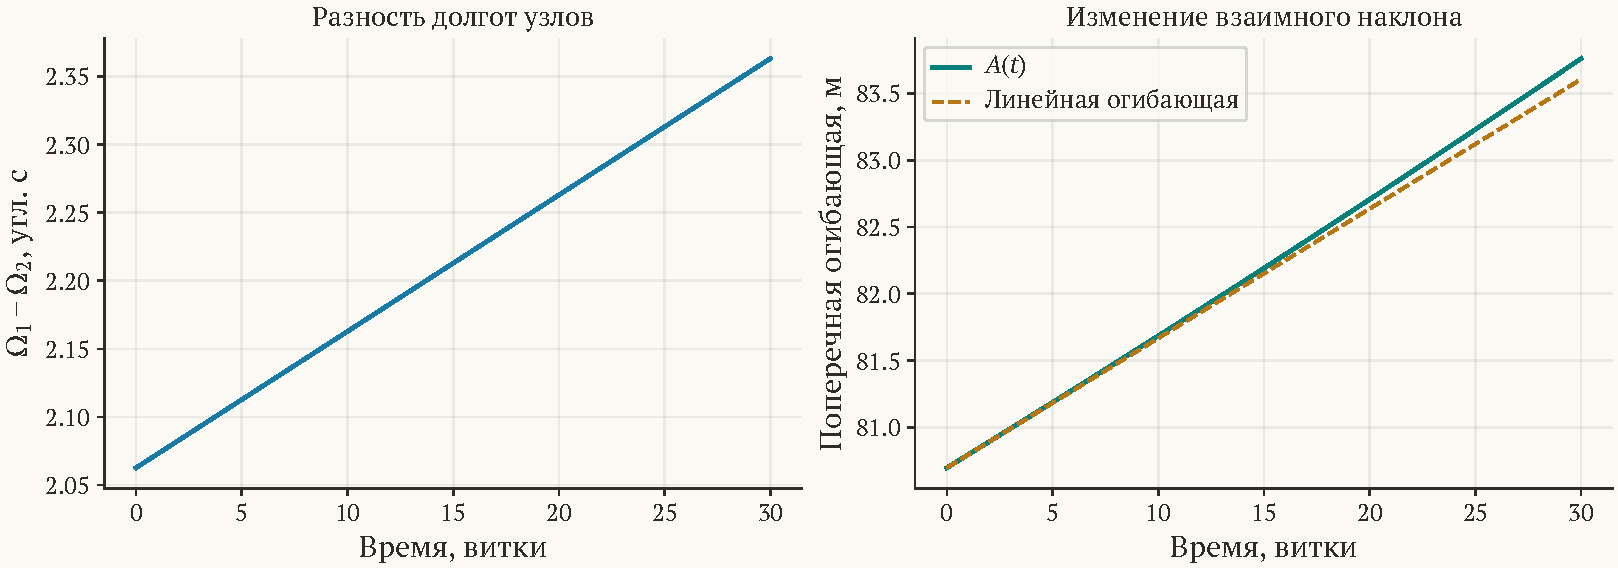
\includegraphics[width=.98\linewidth,height=45mm,keepaspectratio]{images/j2-frequencies-slide.pdf}
\par
\justifying
$A(t)\simeq r_{\rm ref}\sin\Psi(t)$; пунктир --- локальная огибающая $A(t)=m+lt$.
Геометрическая иллюстрация не проверяет полную модель SS.
\end{frame}

\begin{frame}{Сравнение моделей с $J_2$}
\relax
\derivationmathspacing
{\eqcompact\derivationmathspacing
\[
\begin{gathered}
 r_{\rm ref}=7000\ \text{км},\quad i_{\rm ref}=0,\quad
 \omega_{\rm ref}=n\sqrt{1+s},\quad x_i=100\ \text{м},\\[-1pt]
 y_i=\dot x_i=0,\quad \dot y_i=-2\omega_{\rm ref}x_i;
 \quad\text{частота вращения в CW равна }\omega_{\rm ref}.
\end{gathered}
\]
}
\centering
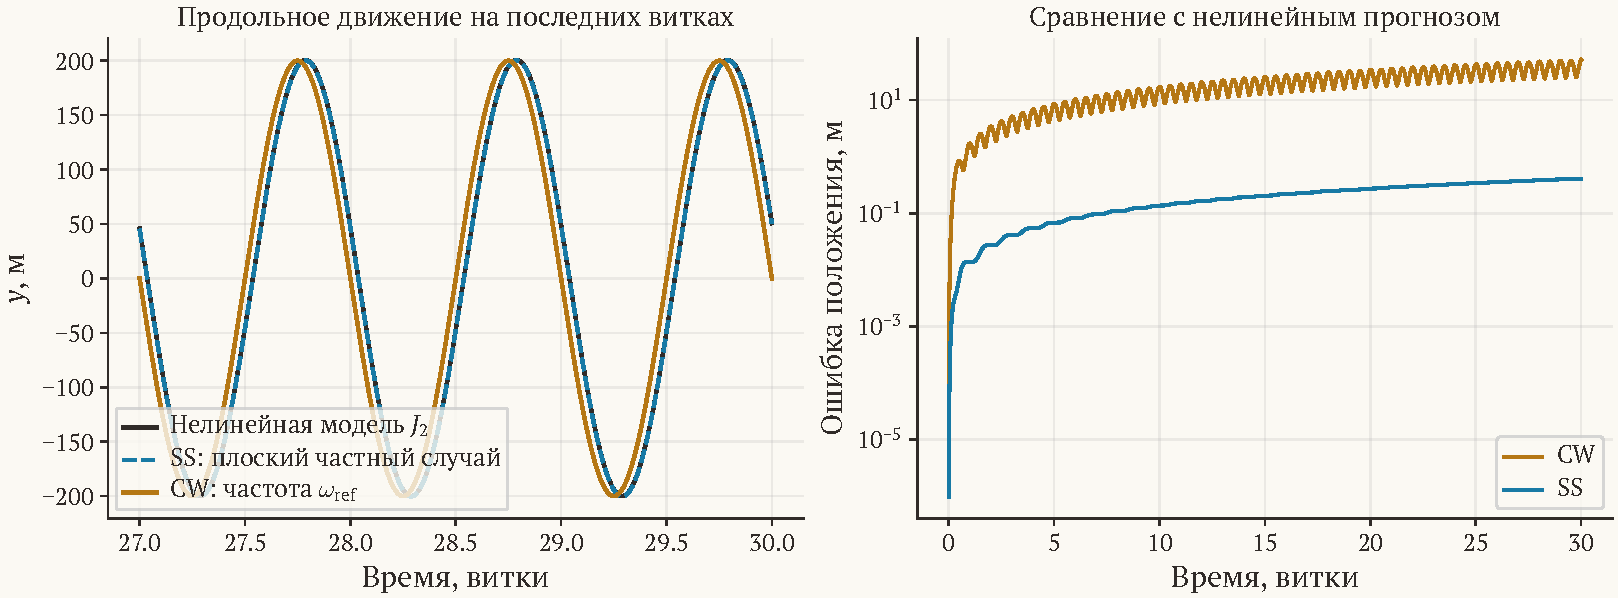
\includegraphics[width=.98\linewidth,height=43mm,keepaspectratio]{images/j2-relative-slide.pdf}
\par
\figcaption{Общие начальные состояния; максимум ошибки за 30 витков: CW --- $50{,}825$ м, SS --- $0{,}408$ м.}
\end{frame}

\begin{frame}{Области применения моделей}
\relax
\derivationmathspacing
\begin{center}
\renewcommand{\arraystretch}{1.25}
\begin{tabular}{@{}>{\raggedright\arraybackslash}p{.19\textwidth}>{\raggedright\arraybackslash}p{.37\textwidth}>{\raggedright\arraybackslash}p{.36\textwidth}@{}}
\textbf{Модель} & \textbf{Динамика} & \textbf{Применимость}\\
\hline
CW & Круговая кеплерова цель & Малое удаление\\
TH / YA & Эллиптическая кеплерова цель & Первый порядок по расстоянию\\
SS & Усреднённые эффекты $J_2$ & Околокруговая орбита\\
Вариационные уравнения & Полная модель сил & Численная матрица перехода
\end{tabular}
\end{center}
\smallskip
\justifying
Во всех линейных моделях требуется малое удаление от опорной траектории.
Относительные орбитальные элементы меняют представление состояния, но не добавляют возмущений.
\end{frame}


% Расчётный пример и уточнение: главы 7--8 методички 7/rendezvous.tex.
\begin{frame}{Пример встречи}
\relax
\derivationmathspacing
При $t_i=0$: индекс $0$ --- цель, $\delta$ --- аппарат минус цель.
{\eqcompact
\[
\begin{aligned}
\ExampleInitialData
\end{aligned}
\]
}
$t_1=0$, $t_2=t_f=1200$ с; начальное расстояние --- $\ExampleInitialDistance$.
$\Delta\vect V_j$ --- в м/с в предманёвренной ОСК.
\begin{columns}[T,onlytextwidth]
\begin{column}{.48\textwidth}
\textbf{Линейная задача}\par\vspace{1pt}
{\eqcompact
\centering
\begin{tabular}{@{}lrrr@{}}
\toprule
&$\Delta V_r$&$\Delta V_t$&$\Delta V_n$\\\midrule
\ExampleLinearComponents
\bottomrule
\end{tabular}\par
}
\end{column}
\begin{column}{.48\textwidth}
\textbf{Задача Ламберта}\par\vspace{1pt}
{\eqcompact
\centering
\begin{tabular}{@{}lrrr@{}}
\toprule
&$\Delta V_r$&$\Delta V_t$&$\Delta V_n$\\\midrule
\ExampleLambertComponents
\bottomrule
\end{tabular}\par
}
\end{column}
\end{columns}
{\eqcompact\par\vspace{2pt}\centering $\theta=\ExampleTransferAngle,\quad p=\ExampleLambertP.$\par}
\end{frame}

\begin{frame}{Встреча в инерциальных координатах}
\relax
\derivationmathspacing
{\centering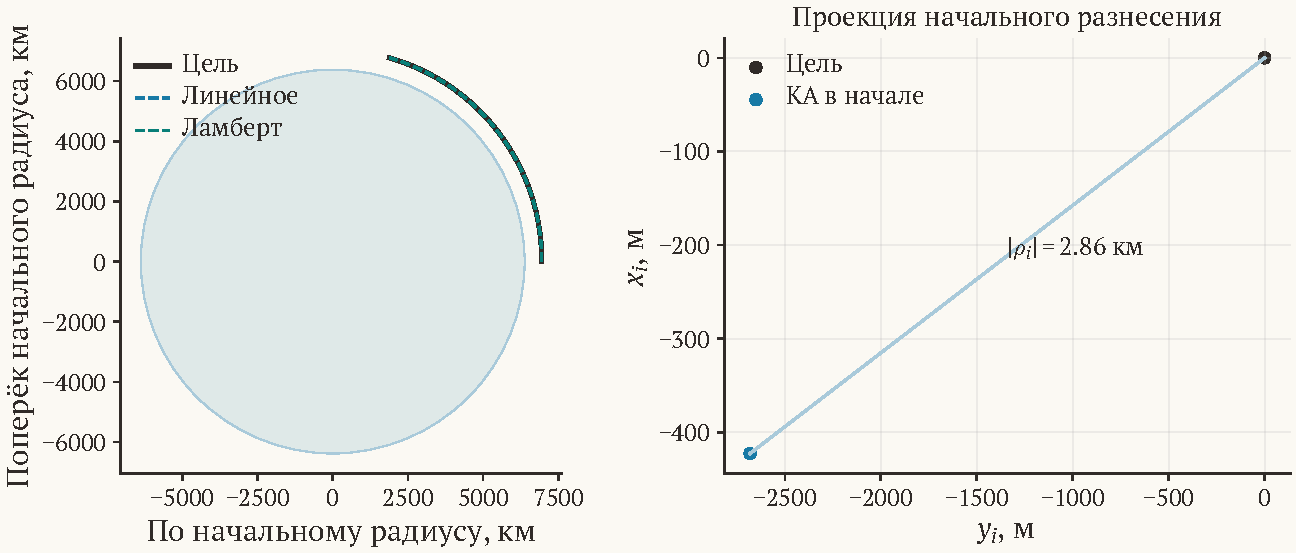
\includegraphics[width=\textwidth,height=52mm,keepaspectratio]{images/rendezvous-orbits-slide.pdf}\par}
Цель и два управляемых перелёта; справа --- начальное разнесение. На орбитальном масштабе близкие траектории почти совпадают.
\end{frame}

\begin{frame}{Траектория встречи}
\relax
\derivationmathspacing
{\eqcompact\derivationmathspacing
\[
 \vect\rho(t)=Q_0(t)^\top\bigl(\vect R_C(t)-\vect R_0(t)\bigr).
\]
}
{\centering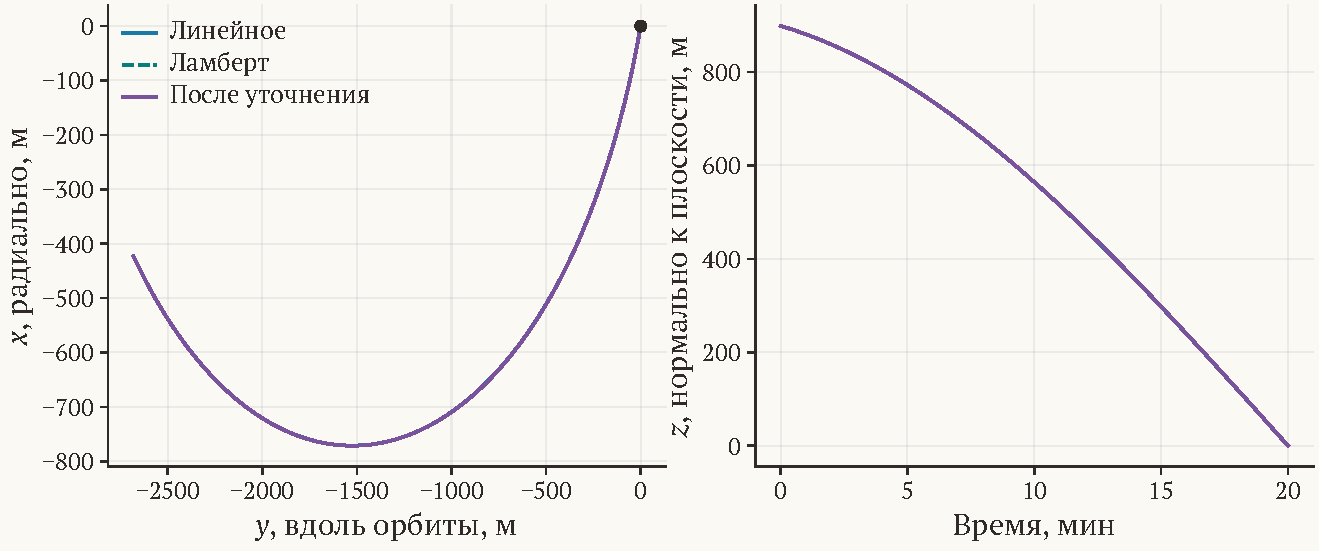
\includegraphics[width=\textwidth,height=46mm,keepaspectratio]{images/rendezvous-relative-slide.pdf}\par}
Одинаковые начальное состояние и $t_f=1200$ с; движение показано в RTN цели.
\end{frame}

\begin{frame}{Нелинейная проверка управления}
\relax
\derivationmathspacing
{\eqcompact\derivationmathspacing
\[
 \dot{\vect R}=\vect V,\qquad
 \dot{\vect V}=-\frac\mu{R^3}\vect R,\qquad
 \vect V_j^+=\vect V_j^-+Q_j\Delta\vect V_j,
\]
\[
 \varepsilon_R=\|\vect R_C(t_f)-\vect R_0(t_f)\|,\qquad
 \varepsilon_V=\|\vect V_C(t_f)-\vect V_0(t_f)\|.
\]
}
Проверка после последнего импульса; ошибки навигации и исполнения не учитываются.
\par\smallskip
{\eqcompact
\centering
\renewcommand{\arraystretch}{1.05}
\setlength{\tabcolsep}{8pt}
\begin{tabular}{@{}lrrr@{}}
\toprule
Решение&$\sum_j\|\Delta\vect V_j\|$, м/с&$\varepsilon_R$, м&$\varepsilon_V$, м/с\\\midrule
\ExampleComparisonRows
\bottomrule
\end{tabular}\par
}
\smallskip
Независимая проверка: $2\cdot10^{-7}$ м и $5\cdot10^{-10}$ м/с. Меньшие ошибки показаны границами.

\end{frame}

\begin{frame}{Уточнение решения}
\relax
\derivationmathspacing
Число импульсов, моменты манёвров и $t_f$ заданы. Уточняются компоненты импульсов в предманёвренных ОСК.
\begin{columns}[T,onlytextwidth]
\begin{column}{.46\textwidth}
{\eqcompact\derivationmathspacing
\[
 \delta\vect y_f^{(k)}=\vect y_t-\vect y_f(\Delta\vect V^{(k)}),
\]
\[
 \mathcal M^{(k)}=\left.
 \frac{\partial\vect y_f}{\partial\Delta\vect V}
                   \right|_{\Delta\vect V^{(k)}},
\]
\[
 \boxed{\mathcal M^{(k)}\delta\vect V^{(k)}
                     =\delta\vect y_f^{(k)}.}
\]
}
Для двух импульсов при невырожденной матрице поправка единственна.
\end{column}
\begin{column}{.51\textwidth}
При $N>2$ и полном строчном ранге:
{\eqcompact\derivationmathspacing
\[
 \min_{\delta\vect V^{(k)}}\sum_{j=1}^N\|\delta\vect V_j^{(k)}\|^2,
 \quad\mathcal M^{(k)}\delta\vect V^{(k)}=\delta\vect y_f^{(k)},
\]
\[
\begin{aligned}
 \delta\vect V^{(k)}={}&(\mathcal M^{(k)})^\top\\[-2pt]
 &\cdot[\mathcal M^{(k)}(\mathcal M^{(k)})^\top]^{-1}
                      \delta\vect y_f^{(k)}.
\end{aligned}
\]
}
Минимизируется норма поправки; сумма норм полных импульсов в этой подзадаче не минимизируется.
\end{column}
\end{columns}
\end{frame}

\begin{frame}{Вычисление текущей производной}
\relax
\derivationmathspacing
Конечное состояние $\vect y_f(\Delta\vect V)$ и строки матрицы записываются в классических элементах $(a,e,\omega,i,\Omega,M)$.
{\eqcompact\derivationmathspacing
\[
 (\mathcal M^{(k)})_{:,\ell}\approx
 \frac{\vect y_f(\Delta\vect V^{(k)}+h_\ell\vect e_\ell)
       -\vect y_f(\Delta\vect V^{(k)}-h_\ell\vect e_\ell)}{2h_\ell}.
\]
}
\begin{columns}[T,onlytextwidth]
\begin{column}{.48\textwidth}
\begin{itemize}
\setlength{\itemsep}{3pt}
\item $h_\ell$ --- приращение компоненты импульса; $\vect e_\ell$ --- единичный столбец.
\item В каждом прогнозе строятся ОСК всех манёвров.
\item Углы продолжаются около одной локальной ветви.
\end{itemize}
\end{column}
\begin{column}{.49\textwidth}
Шаг проверяют расчётом при $h_\ell/2$; в примере $h_\ell=10^{-3}$ м/с.
\par\smallskip
При $\Delta\vect V=0$ производная сводится к блокам $\Phi B$ на $\vect y_0(t)$.
\par\smallskip
При ненулевых импульсах матрица пересчитывается: меняются орбиты и предманёвренные базисы.
\end{column}
\end{columns}
\end{frame}

\begin{frame}{Обновление управления и остановка}
\relax
\derivationmathspacing
{\eqcompact\derivationmathspacing
\[
 \Delta\vect V^{(k+1)}=\Delta\vect V^{(k)}
                  +\alpha_k\delta\vect V^{(k)},\qquad0<\alpha_k\le1.
\]
}
При росте масштабированной конечной невязки уменьшают $\alpha_k$. Для решения строки состояния масштабируют; для остановки проверяют положение и скорость:
{\eqcompact\derivationmathspacing
\[
 \varepsilon_R\le\varepsilon_{R,\rm req},\qquad
 \varepsilon_V\le\varepsilon_{V,\rm req}.
\]
}
{\eqcompact
\centering
\renewcommand{\arraystretch}{1.05}
\setlength{\tabcolsep}{8pt}
\begin{tabular}{@{}rrrr@{}}
\toprule
Итерация&$\varepsilon_R$, м&$\varepsilon_V$, м/с&$\sum_j\|\Delta\vect V_j\|$, м/с\\\midrule
\ExampleCorrectionRows
\bottomrule
\end{tabular}\par
}
\smallskip
В примере заново вычисляются шесть столбцов $\mathcal M^{(k)}$ и принимается полный шаг $\alpha_k=1$. Малый шаг при большой невязке не означает выполнения конечного условия.
\end{frame}

\begin{frame}{Уточнение расчётного примера}
\relax
\derivationmathspacing
{\centering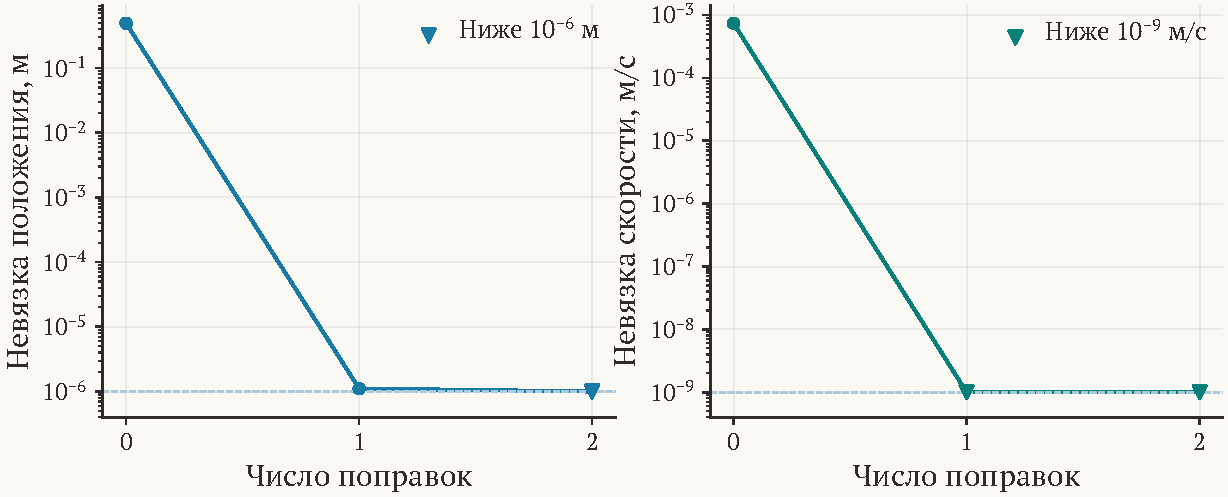
\includegraphics[width=\textwidth,height=52mm,keepaspectratio]{images/rendezvous-convergence-slide.pdf}\par}
Одна поправка: $\varepsilon_R$ уменьшается с $0{,}492$ м до $1{,}1\cdot10^{-6}$ м. Уточнение встречи не устанавливает минимальность характеристической скорости.
\end{frame}


\begin{frame}{Литература}
\relax
\setbeamertemplate{bibliography item}{\insertbiblabel}
\begin{thebibliography}{9}
\bibitem{BMW}
Bate R.~R., Mueller D.~D., White J.~E.
\textit{Fundamentals of Astrodynamics}. Dover, 1971.
\S\,5.2, 5.4, 9.4.1.
\bibitem{Baranov}
Баранов А.~А. \textit{Маневрирование космических аппаратов
в окрестности круговой орбиты}. М.: Спутник+, 2016. Гл.~1--2.
\bibitem{Chinyaev}
Чиняев В.~Н., Кузнецов А.~А., Чугунов В.~В.
\textit{Ускоренный алгоритм решения задачи встречи космических аппаратов на возмущённых эллиптических орбитах}.
Предоставленная автором рукопись, 2025.
\bibitem{CW1960}
Clohessy W.~H., Wiltshire R.~S.
\href{https://doi.org/10.2514/8.8704}{Terminal Guidance System for Satellite Rendezvous} //
\textit{Journal of the Aerospace Sciences}. 1960. Vol.~27. P.~653--658, 674.
\end{thebibliography}
\end{frame}

\begin{frame}{Литература}
\relax
\setbeamertemplate{bibliography item}{\insertbiblabel}
\begin{thebibliography}{9}
\setcounter{enumiv}{4}
\bibitem{YA2002}
Yamanaka K., Ankersen F.
\href{https://doi.org/10.2514/2.4875}{New State Transition Matrix for Relative Motion on an Arbitrary Elliptical Orbit} //
\textit{JGCD}. 2002. Vol.~25, no.~1. P.~60--66.
\bibitem{SS2002}
Schweighart S.~A., Sedwick R.~J.
\href{https://doi.org/10.2514/2.4986}{High-Fidelity Linearized $J_2$ Model for Satellite Formation Flight} //
\textit{JGCD}. 2002. Vol.~25, no.~6. P.~1073--1080.
\bibitem{London1963}
London H.~S. Second Approximation to the Solution of the Rendezvous Equations // \textit{AIAA Journal}. 1963. Vol.~1. P.~1691--1693.
\bibitem{Karlgaard2003}
Karlgaard C.~D., Lutze F.~H. Second-Order Relative Motion Equations // \textit{JGCD}. 2003. Vol.~26. P.~41--49.
\bibitem{Gim2003}
Gim D.~W., Alfriend K.~T. State Transition Matrix of Relative Motion for the Perturbed Noncircular Reference Orbit // \textit{JGCD}. 2003. Vol.~26. P.~956--971.
\end{thebibliography}
\end{frame}
\end{document}
